\chapter{Results and Discussion}
\label{ch:randd}
\graphicspath{{image_directory/resultsanddiscussion/}}

	The following results are organised as the following: simple theoretical road networks used to test numerical features, road sections from two real-world locations showing the application of this model to real situations, and an analysis of various simulation times. 
	
\section{Simple Road Tests}

	To begin using the model, the most simple road networks are to be tested. Is it useful to test over-simplified and somewhat unrealistic networks to show the working features of the probabilistic network model and some simple features such as the source and sink roads in action. Here a simple single road and a network, proposed by Bretti, Natalini, and Piccoli \cite{Bretti07}, known as the traffic circle resembling a common roundabout.
	
\subsection{Single Road Segment}
\label{randd:singleroad}

	The most simple network tested is a straight road with no junctions, made up of a single road segment that is both a source and a sink. The junction solver is not called as there are no defined junctions, hence this test can be executed very quickly due to the simple simulation process. 
	\\ \\ 
	This simple network is useful to expose individual features of the solver, such as the higher order WENO reconstruction methods. As described in Section \ref{sec:HRS} and given explicitly in Appendix \ref{ap:WENOreco}, the 5$^{th}$ and 7$^{th}$ order schemes are available as reconstruction methods. The 7$^{th}$ order method is equivalent by process to the 5$^{th}$ and 3$^{rd}$, with the addition of steps to preserve the monotonic bounds of each cell reconstruction \cite{BalsaraShu00},\cite{Suresh97}. Figure \ref{fig:randd:single:7thOrder} shows the 7$^{th}$ order density profile solution for the single road with 5$^{th}$ order as a reference. The yellow line shows the density profile for the unbounded-7$^{th}$ order WENO scheme. The solution following the 10$^{th}$ time step becomes \emph{numerically} unbounded for the unbounded-7$^{th}$ order WENO scheme. This shows that the procedure presented in Appendix \ref{ap:WENOreco}, for the general $(2k-1)^{th}$ scheme cannot be extended to $k\ge4$ without extra methodology applied such as the monotonicity preserving bounds \cite{BalsaraShu00}. This figure also highlights the advantage of the 7$^{th}$ order scheme over the 5$^{th}$, in terms of capturing density jumps to a higher accuracy. The 5$^{th}$ order scheme actually predicts a jump in density earlier than the main density drop, a high density clustering of fast moving cars at the front of the stream. This is unrealistic, and predicted better by the 7$^{th}$ order scheme.

	\begin{figure}
    		\centering
        		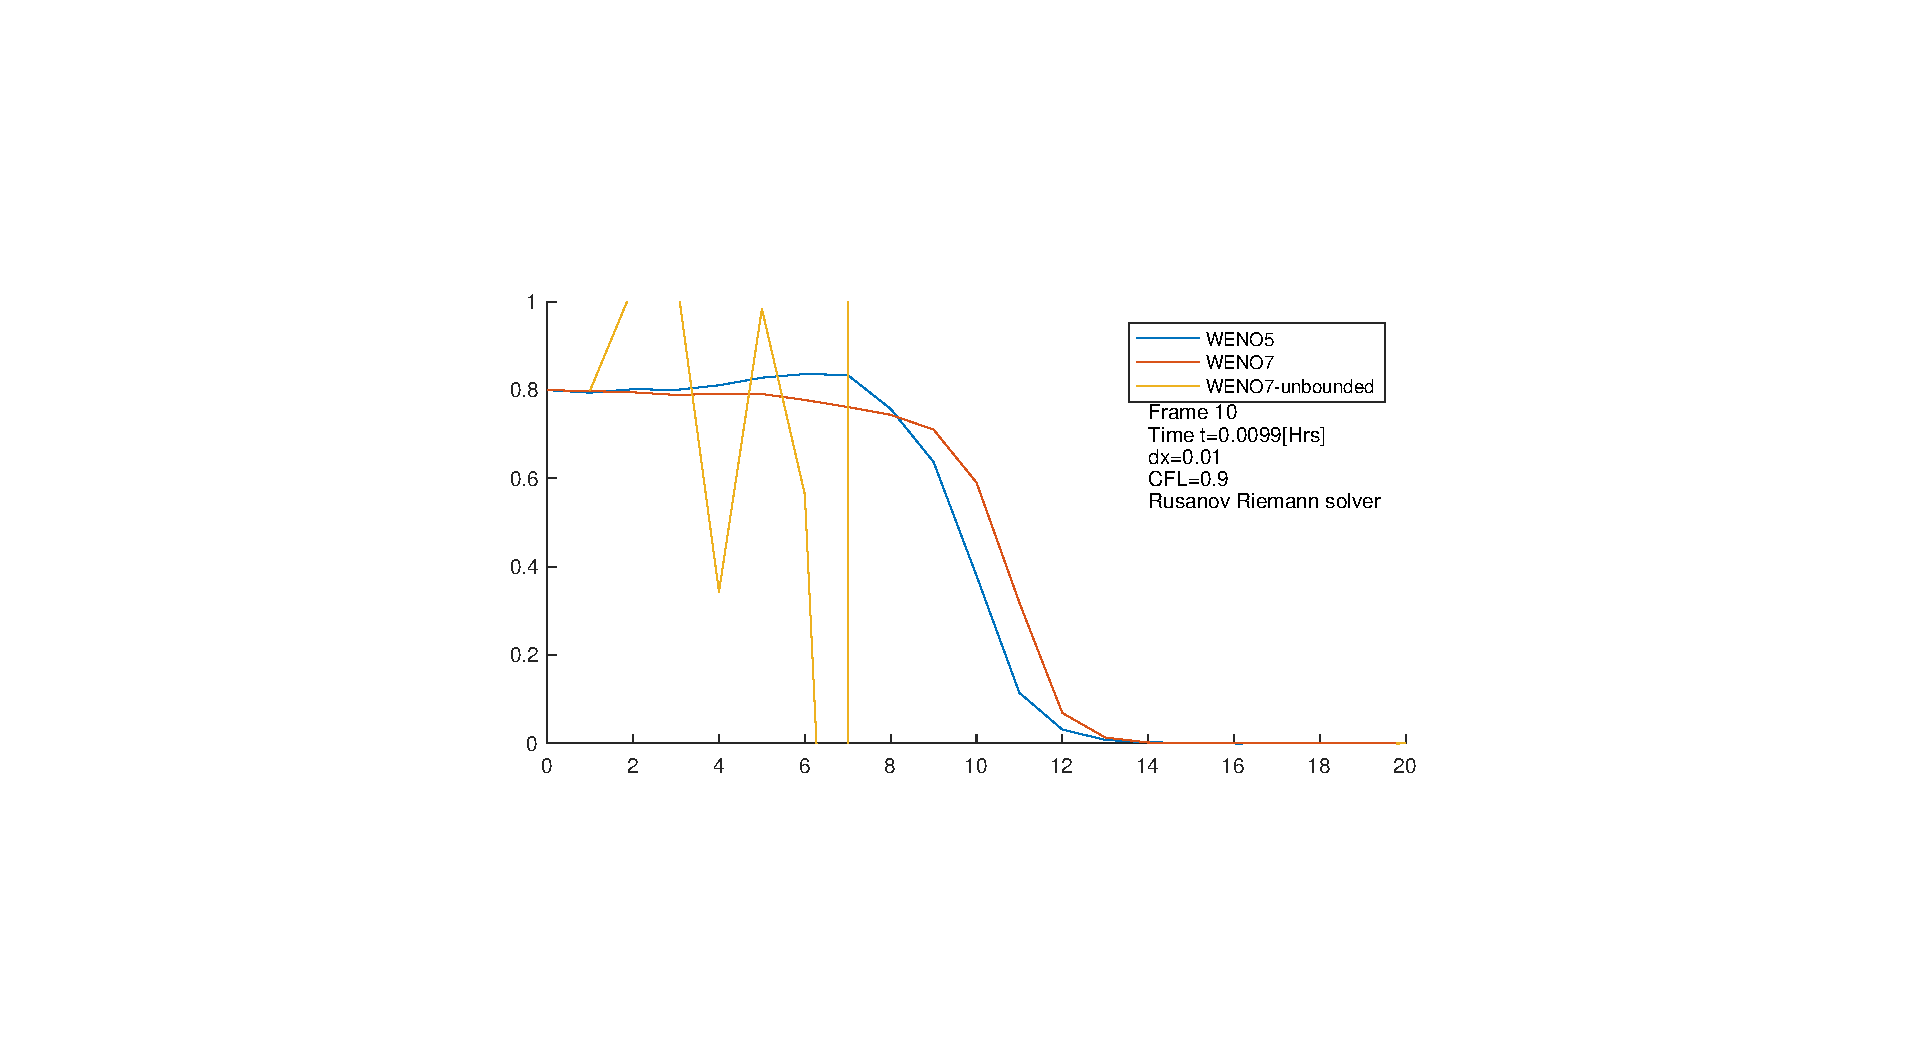
\includegraphics[trim=240 130 230 130,clip,width=0.7\textwidth]{SingleRoad_W7.pdf}
		\caption[Single Road : 7th order WENO]{The scheme used for 5th and 3rd order WENO reconstruction cannot be extended to 7$^{th}$ order without monotonic bounding applied. The unbounded solution is highly modulated, and becomes numerically unbounded after 10 time steps.}
		\label{fig:randd:single:7thOrder}
	\end{figure}

\subsection{Traffic Circles}
\label{randd:trafficcircles}

	The following simulations have reproduced the traffic-circles network and parameters from \cite{Bretti07}, with 8 roads joined by 4 junctions (as shown in Figure 9 of \cite{Bretti07}). Unless otherwise stated in the figure legend, the simulation settings for the results and following discussion are d$x=0.01$, $CFL=0.9$, $2^{nd}$ order reconstruction and Lax-Friedrichs Riemann solver. The defined inlet density from the left and right are 0.25 and 0.4 respectively, this feeds into the four central roads which can be shown by the jump in density along the four internal roads and top and bottom outlet roads, shown in all Figures \ref{fig:randd:traffic_circles_reco}, \ref{fig:randd:traffic_circles_riemann}, \ref{fig:randd:traffic_circles_dx}. 
	\\ \\
	It is expected that high order spatial reconstruction results in a more accurate prediction of jumps in traffic density, however  such simulation parameters as in Figure \ref{fig:randd:traffic_circles_reco}, there is no obvious advantage of the 3$^{rd}$ order WENO over 2$^{nd}$ order TVD reconstruction. The parameter $q_1=0.5$ describes equal flow joining and leaving the traffic circle at available junctions. A result of this some density will always remain in the central roads and the density profile will become smoother where the effect of spatial reconstruction is not as significant.
	\\ \\
	One major fault of the model concerning the numerical flux calculation is the definition of certain parameters used in calculations from Section \ref{sec:RSFC}. This is concluded from Figure \ref{fig:randd:traffic_circles_riemann} where the Rusanov, Murman-Roe and HLL solvers all appear to give an identical solution. The Lax-Friedrichs solution differs from the other solvers but in a less accurate manner in terms of shock resolution.
	\\ \\ 
	Another highly influential parameter in the resolution of density jumps is the spatial resolution $dx$, of which each road segment is split into cells of this size where the density profile is resolved. Figure \ref{fig:randd:traffic_circles_dx} gives another solution to the traffic circle network, with the values of $dx$ for each grid given in the caption. As expected the coarser resolution smooths out density jumps, whereas finer will capture a stronger shock, which is clear from this figure. The coarse and fine simulations give smooth density profiles in comparison to the medium solution which gives a slightly more oscillatory jump. 
	\\ \\
	Another aspect of the flow modelling that is analysed through the traffic circles network is the MUSCL reconstruction slope limiters, discussed in Section \ref{sec:HRS} and given in Appendix \ref{ap:MUSCLreco}. All of the 15 listed slope limiters are applied and solutions shown in Figure \ref{fig:randd:traffic_circles:limiters}, where the top row and bottom row respectively represent limiters applied to the 2$^{nd}$ and 3$^{rd}$ order MUSCL reconstructions. It is immediately clear that the 3$^{rd}$ order MUSCL reconstructed solutions are more oscillatory with all limiters. Of the 2$^{nd}$ order reconstructed solutions, the smoothest profiles arise from the Monotonised Central, UMIST and VanLeer limiters. The VanAlbada2 limiter is numerically unstable for both MUSCL schemes, the solution becomes so oscillatory that after sufficient time steps it is numerically unbounded. This may arise as a result of the violation of Sweby's TVD region \cite{Sweby84} for slope limiters, see Appendix Figure \ref{fig:app:slopelims}.

	\begin{figure}
    		\centering
        		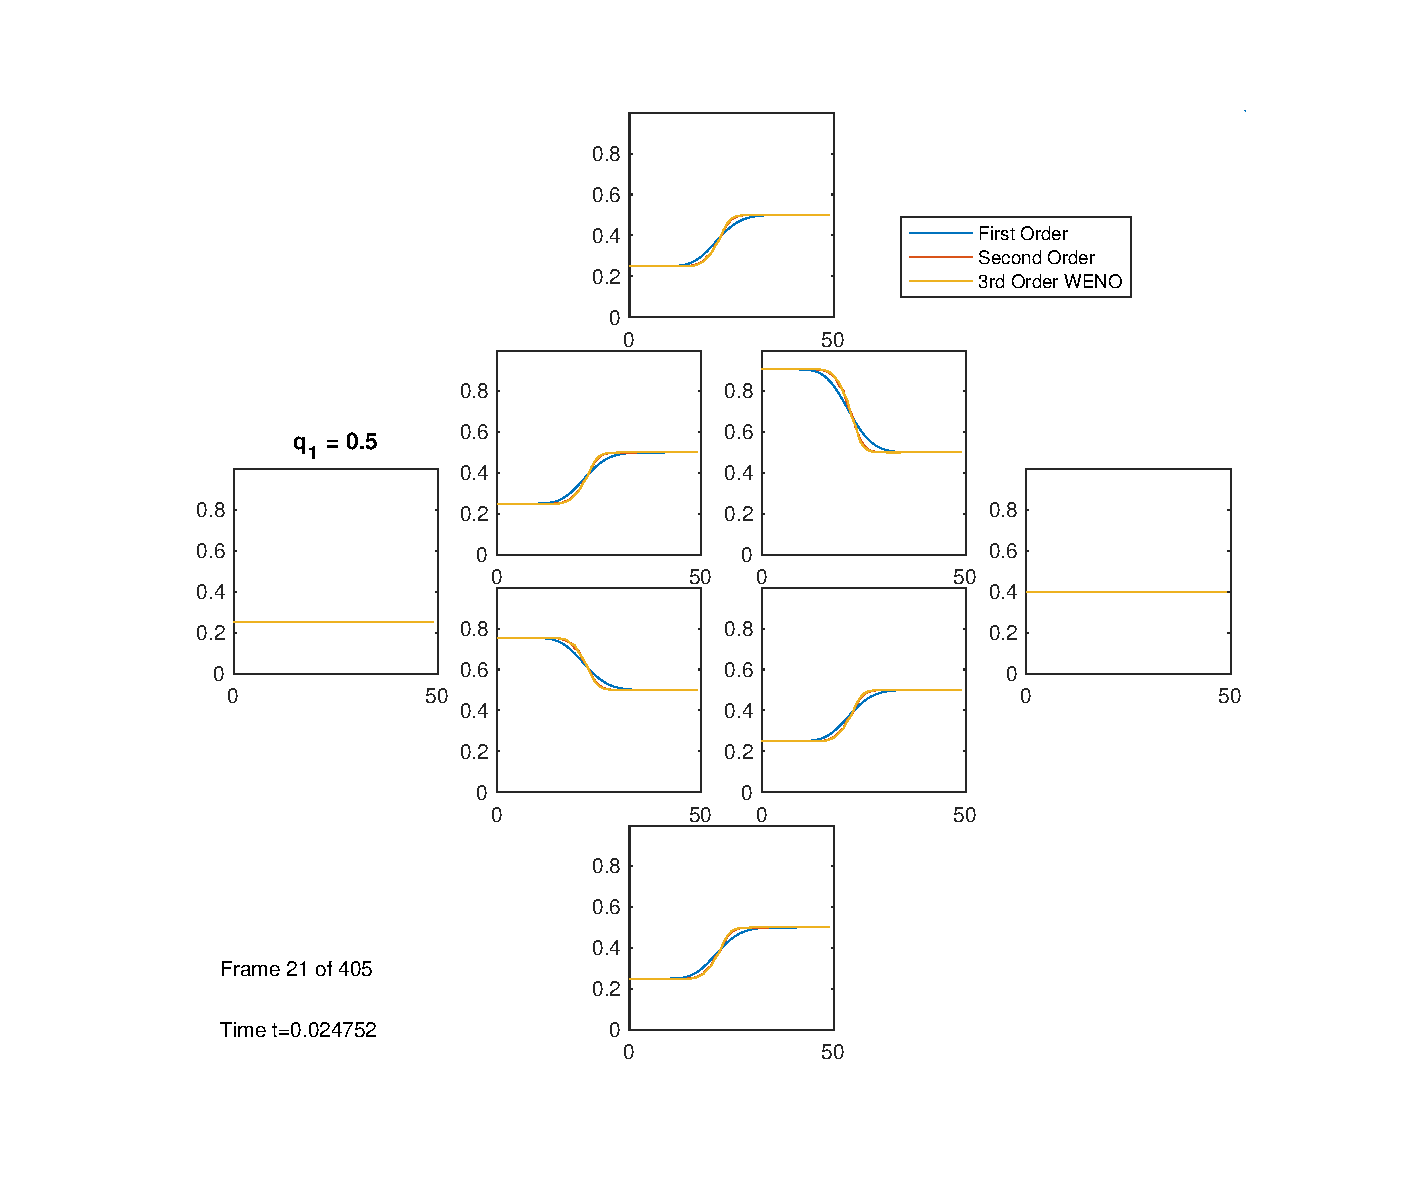
\includegraphics[trim=80 50 80 50,clip,width=0.78\textwidth]{trafficCircles1.pdf}
		\caption[Traffic Circles : Reconstruction methods]{Spatial reconstruction influence, lower order reconstruction smooths out local discontinuities.}
		\label{fig:randd:traffic_circles_reco}
	\end{figure}
	\begin{figure}
    		\centering
        		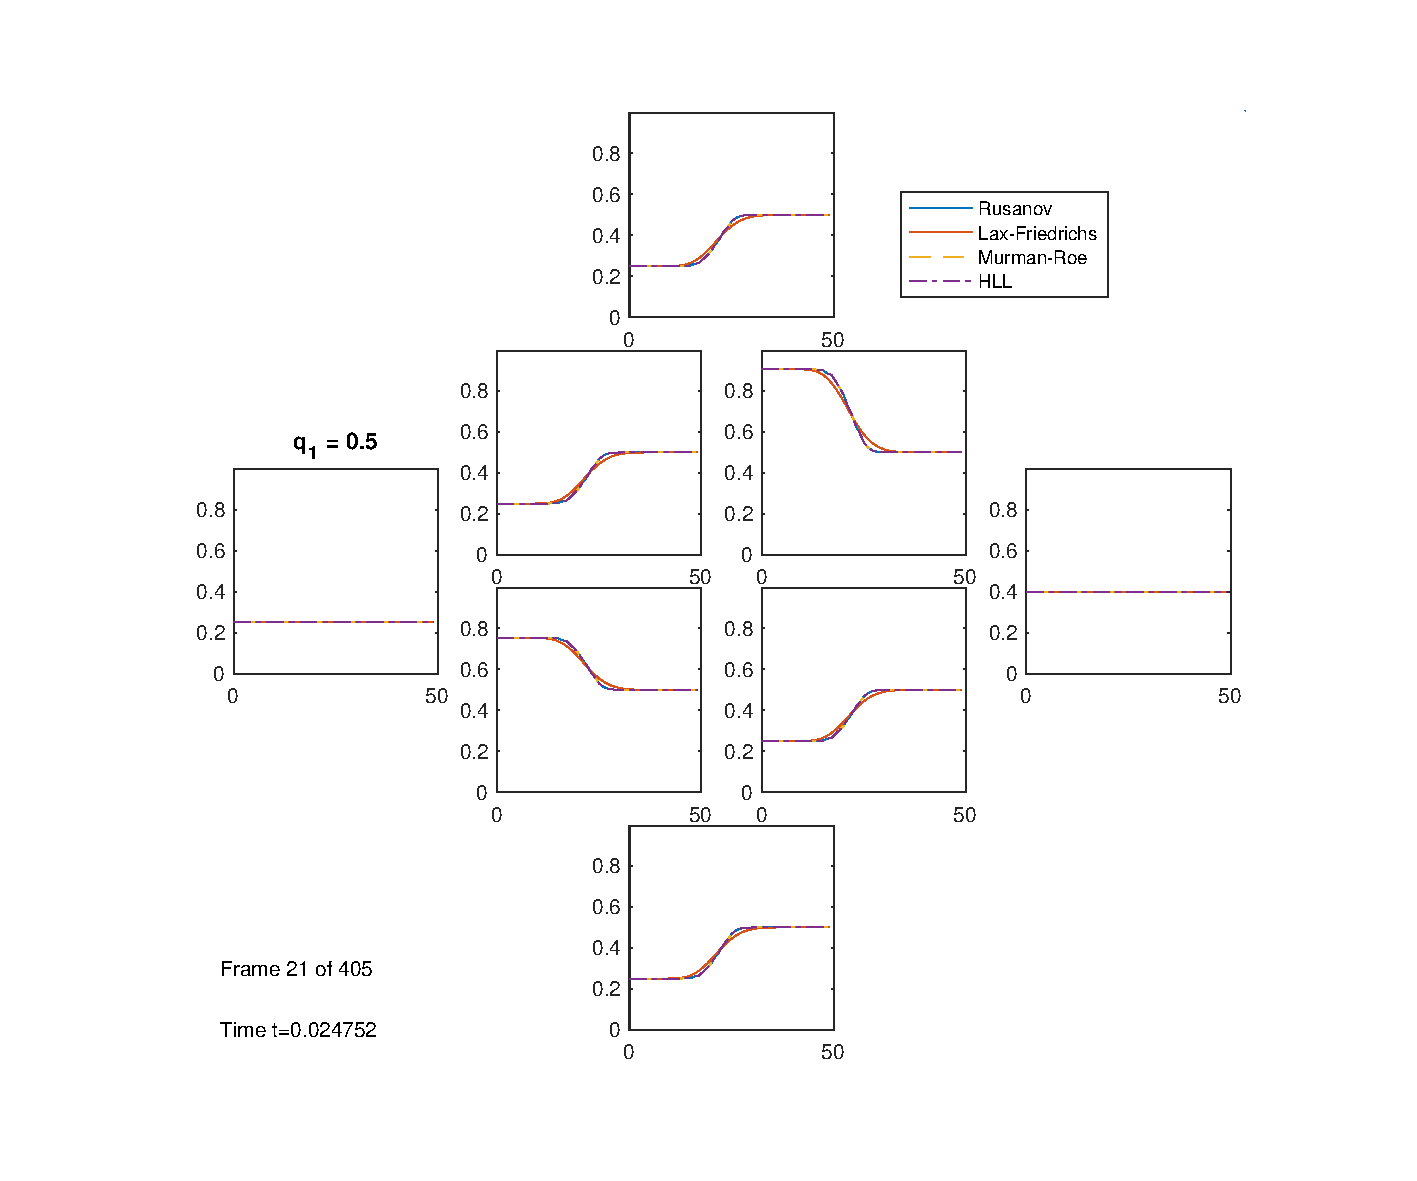
\includegraphics[trim=80 50 80 50,clip,width=0.75\textwidth]{trafficCircles2.pdf}
		\caption[Traffic Circles : Riemann solvers]{Varying the Riemann problem solution method, showing the equivalence of Rusanov, HLL and Murman-Roe.}
		\label{fig:randd:traffic_circles_riemann}
	\end{figure}
	\begin{figure}
    		\centering
        		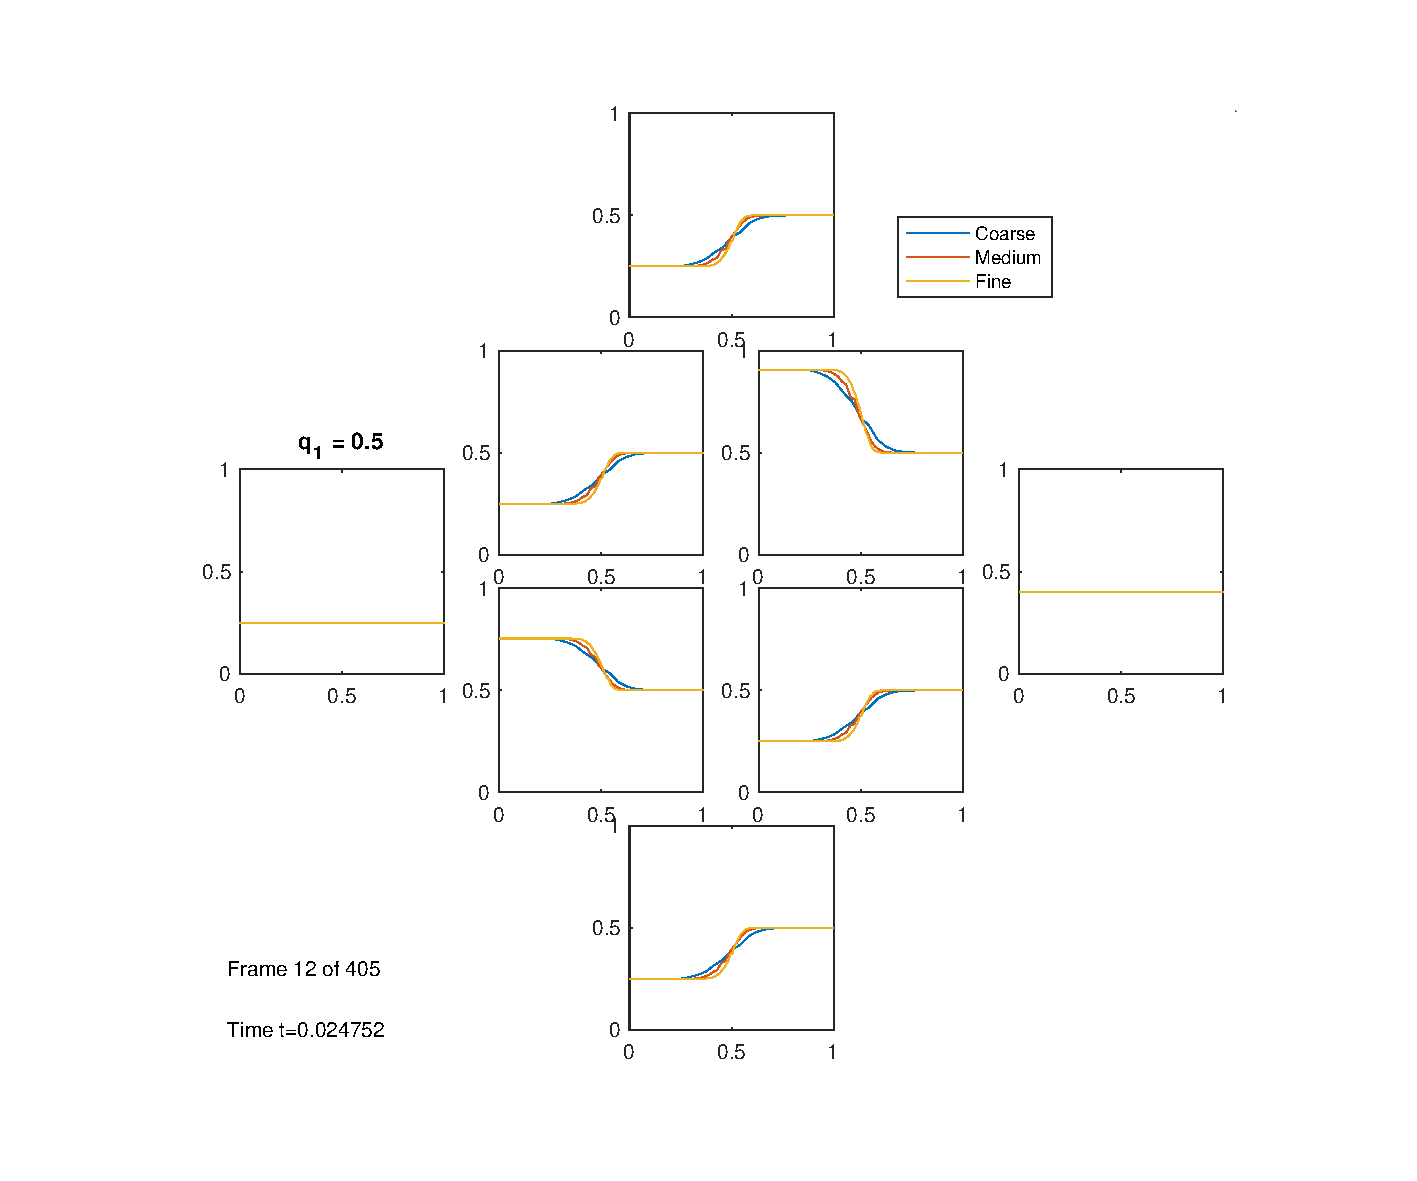
\includegraphics[trim=80 50 80 50,clip,width=0.75\textwidth]{trafficCircles3.pdf}
		\caption[Traffic Circles : Spatial refinement]{Coarse to fine respectively represents $dx=0.02,0.01,0.005$. Increasing the spatial increment causes discontinuities to be resolved more accurately, coarse grids dissipate the density shock.}
		\label{fig:randd:traffic_circles_dx}
	\end{figure}
	\begin{figure}
    		\centering
        		\includegraphics[trim=140 85 135 70,clip,width=\textwidth]{trafficcircles_Limiters.pdf}
		\caption[Traffic Circles : MUSCL limiters]{Various slope limiters applied to MUSCL reconstruction on the traffic circle case. The top and bottom rows represent the density solution on the leftmost inlet road with second and third order MUSCL reconstructions respectively. The VanAlbada2 limiter becomes numerically unbounded after 10 and 35 time steps for 2nd and 3rd order reconstructions respectively.}
		\label{fig:randd:traffic_circles:limiters}
	\end{figure}

\section{Real Road Networks}

	Following the theoretical networks used to test the models numerical and probabilistic capabilities, these sections show how the simulations work when reproducing traffic behaviour on real road network sections. The Piazza dei Re Di Roma roundabout in southeast Rome, and a common UK motorway junction taken from the M1 near Leeds.

\subsection{Re Di Roma Roundabout}

	This road section is studied in \cite{Bretti07}, and resembles a more realistic traffic circle as in Section \ref{randd:trafficcircles}. Figure \ref{fig:randd:RDR:map} shows the network surrounding the roundabout from Google Maps. As this network is real, the postprocessing involving a real road network simulation needs to be more aesthetic than density profile plots. Figure \ref{fig:randd:rediroma} shows the result from an initial simulation using the Re Di Roma roundabout. This figure shows the density not as a distribution but through colour of a physical diagram of the network, the MATLAB code used to generate these figures is given in Appendix \ref{code:ReDiRoma}. Frames from this initial simulation are used to generate the animation \emph{ReDiRoma.mp4}. The parameters used for this simulation result in the solution developing (Figure \ref{fig:randd:rediromaA}) and reaching a steady state (Figure \ref{fig:randd:rediromaB}). These results use first order cell reconstruction with the Lax-Friedrichs Riemann solver. The following results test other numerical methods on the Re Di Roma network, only showing the solution for the central roundabout in polar coordinates the density is shown by the distance from the black circle.
	\\ \\
	As this real network has road segments of irregular length, choosing an arbitrary spatial increment $dx$ can cause the postprocessing to be out of sync when comparing two solutions. Figure \ref{fig:randd:rediroma:grids} shows the roundabout density solution with different spatial resolutions, the coarse simulation is slightly out of sync due to the length of the road network not being divisible into an integer number of cells. For this reason, the coarse profile is smoothed over the density jumps resulting from traffic coming in to the roundabout from source roads. The drops in density are equivalently from sink roads leaving the roundabout. The fine simulation predicts the density jump locations more accurately than both medium and fine. The south-southwest region of the roundabout has an increase of density, shown by the fine and medium solutions, however the coarse solution smooths this small increase in density so much that it could be interpreted differently if analysed without the finer solutions to compare to.
	\\ \\
	The analysis of reconstruction methods on the Re Di Roma roundabout is shown at two stages during the simulation in Figure \ref{fig:randd:rediroma:reco}. This physical postprocessing method makes identifying shock capturing accuracy difficult, however is used to show the application to real networks. On the south of the roundabout (left figure), it is evident that the 3$^{rd}$ order WENO reconstruction captures a stronger shock than the second order and first order as expected. It is useful to know these reconstruction methods are behaving as expected even when embedded in a large program that is solving a complicated process defined on an equally complicated real road network. Later in the simulation (right figure) the solution is becoming more smooth so the effect of reconstruction is not as significant. 
	\\ \\
	We have already seen from simulations on the traffic circle, and in Figure \ref{fig:randd:traffic_circles_riemann}, that the choice of Riemann solver has little influence. Figure \ref{fig:randd:rediroma:riem} shows this is also the case for the Re Di Roma roundabout case. The solution for the HLL and Murman-Roe solvers are equivalent with the Lax-Friedrichs solution differing only very slightly. It is clear that the definition of Riemann solvers in traffic flow network modelling simulations needs to be decided more carefully. 
	
	\begin{figure}
    		\centering
        		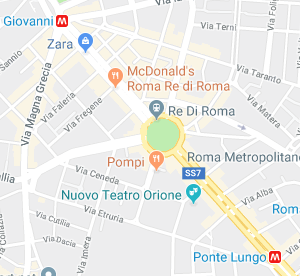
\includegraphics[trim=0 0 0 0,clip,width=0.57\textwidth]{RDR_map.png}
		\caption[Re Di Roma : Junction area map]{Central Rome roundabout network. \emph{Google Maps, 2019.}}
		\label{fig:randd:RDR:map}
	\end{figure}

	\begin{figure}
  		\centering
  		\subfloat[Developing flow]{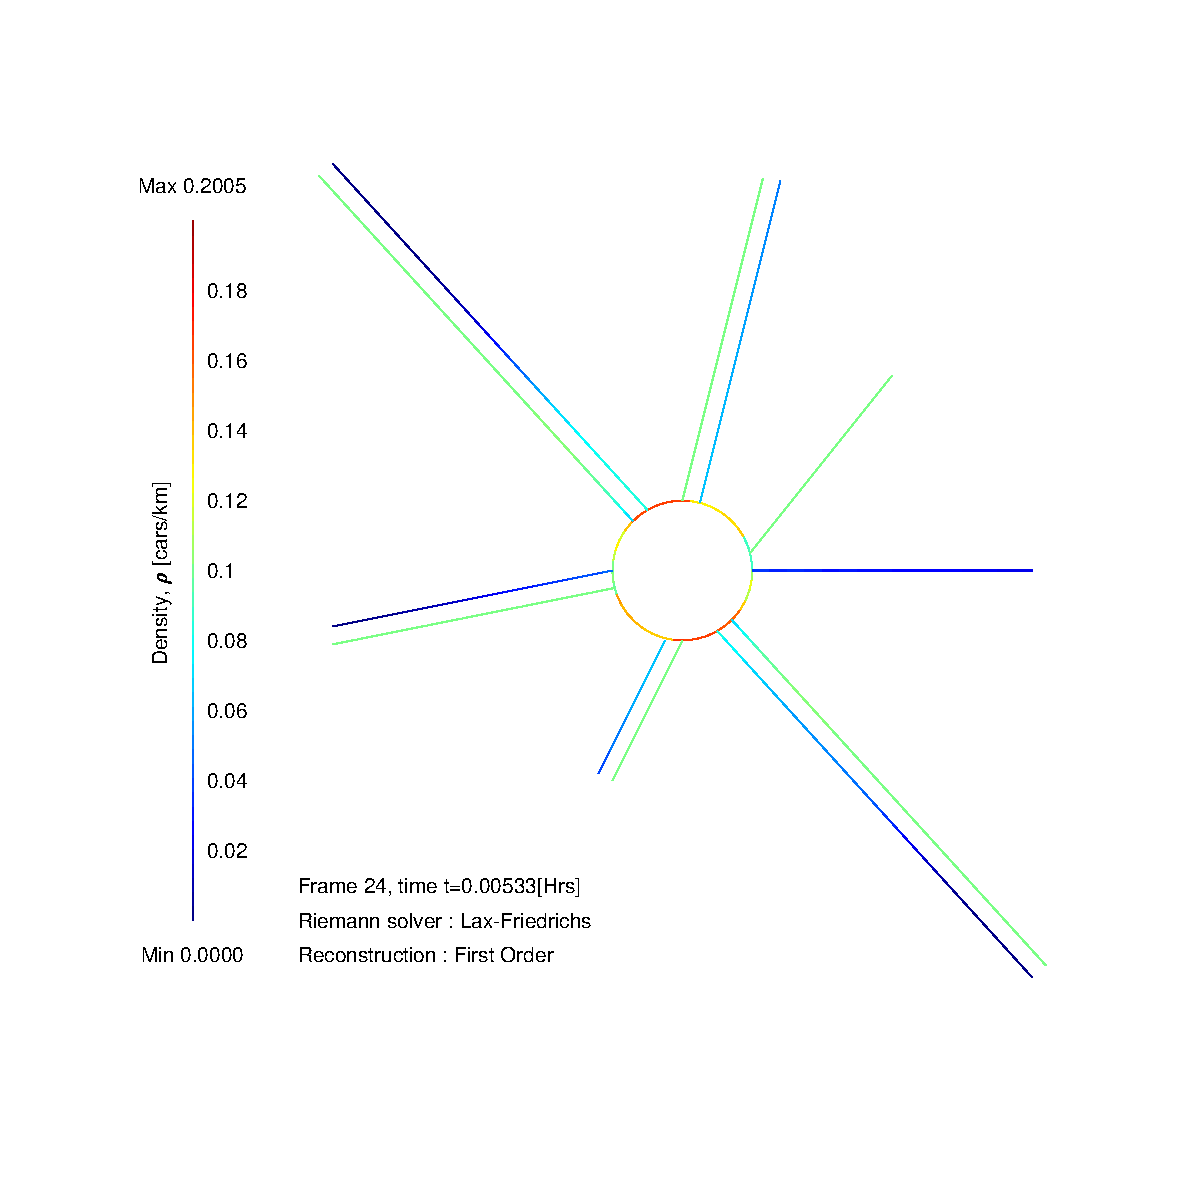
\includegraphics[trim=135 95 64 75,clip,width=0.45\textwidth]{ReDiRoma2.pdf}\label{fig:randd:rediromaA}}
  		\hfill
  		\subfloat[Steady traffic distribution]{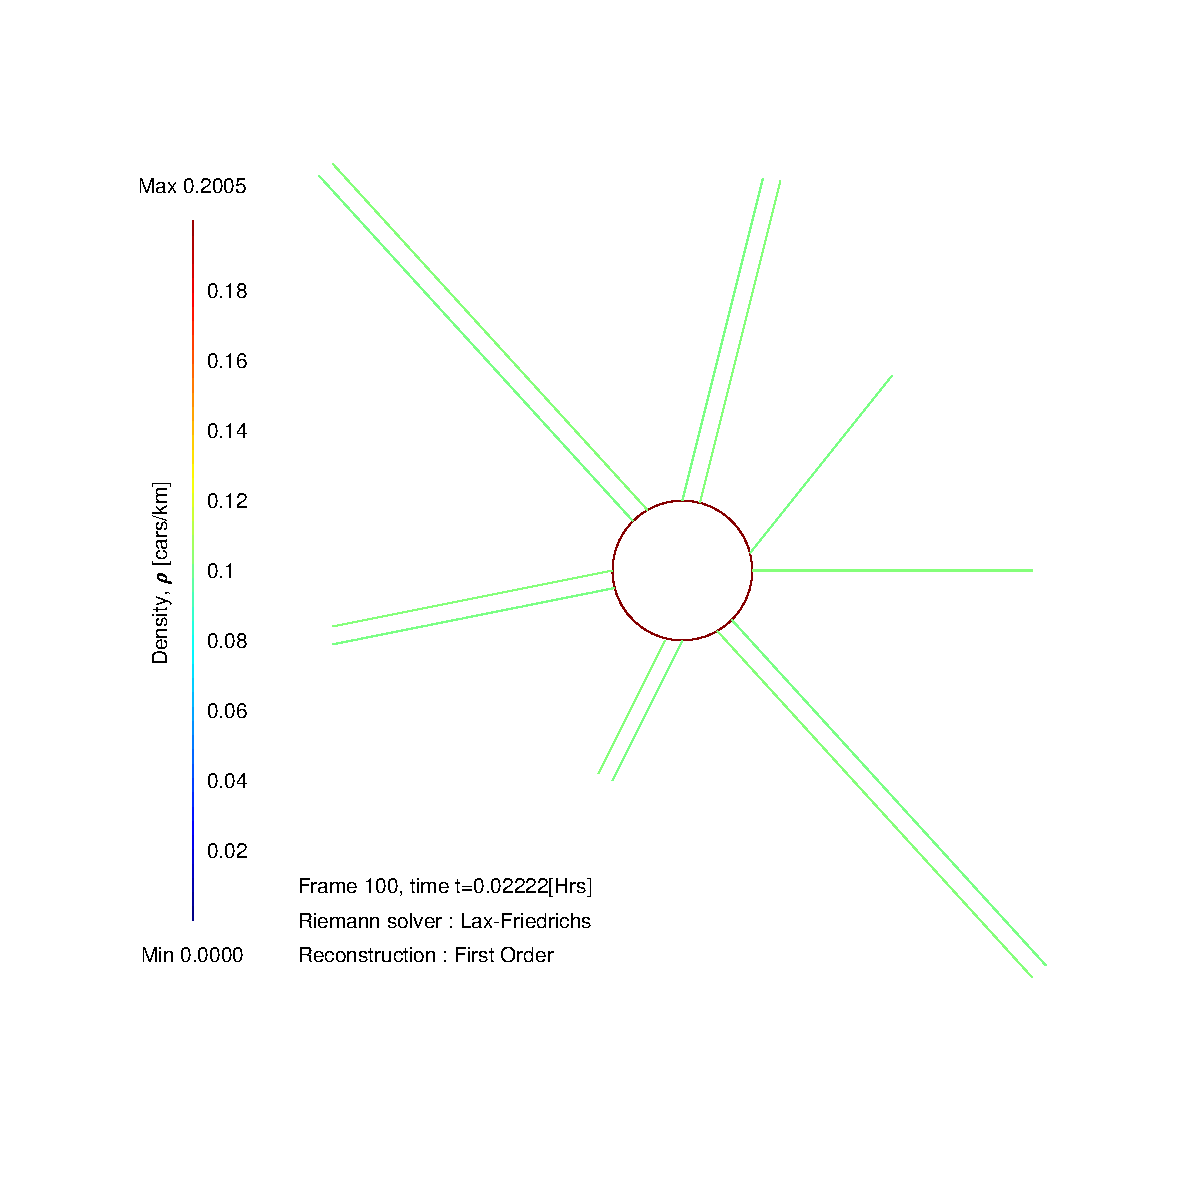
\includegraphics[trim=65 95 64 75,clip,width=0.53\textwidth]{ReDiRoma3.pdf}\label{fig:randd:rediromaB}}
  		\caption[Re Di Roma : Density line contour]{From the initially empty distribution, traffic flows towards the roundabout (a) and reaches a steady density profile (b).  \label{fig:randd:rediroma}}
	\end{figure}
	
	\begin{figure}
    		\centering
        		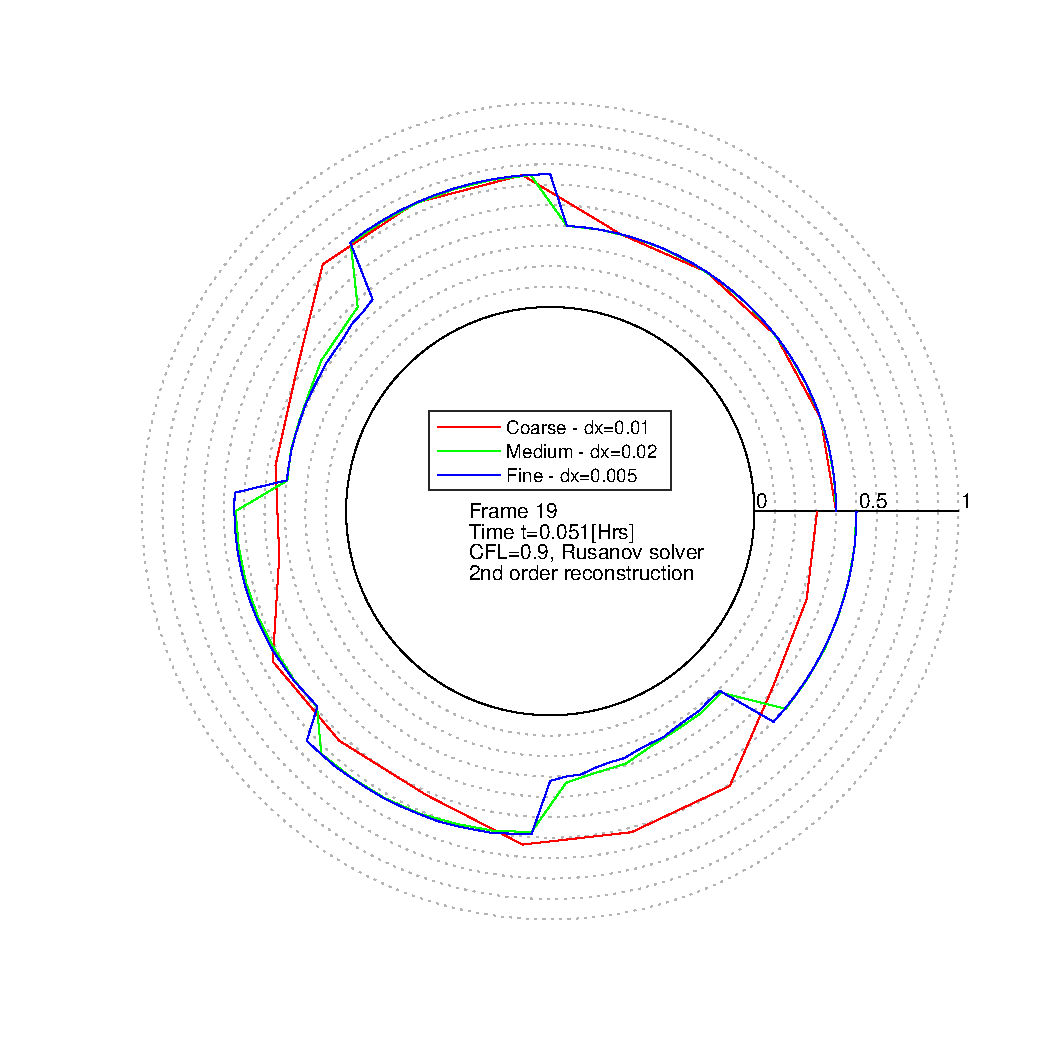
\includegraphics[trim=60 60 40 40,clip,width=0.8\textwidth]{ReDiRoma_grid.pdf}
		\caption[Re Di Roma : Grid resolution]{As expected the finer grid resolves jumps in density from oncoming roads well, the coarse grid is such that it smooths or even misses density jumps completely due to the resolution of the simulation.}
		\label{fig:randd:rediroma:grids}
	\end{figure}
	
	\begin{figure}
    		\centering
        		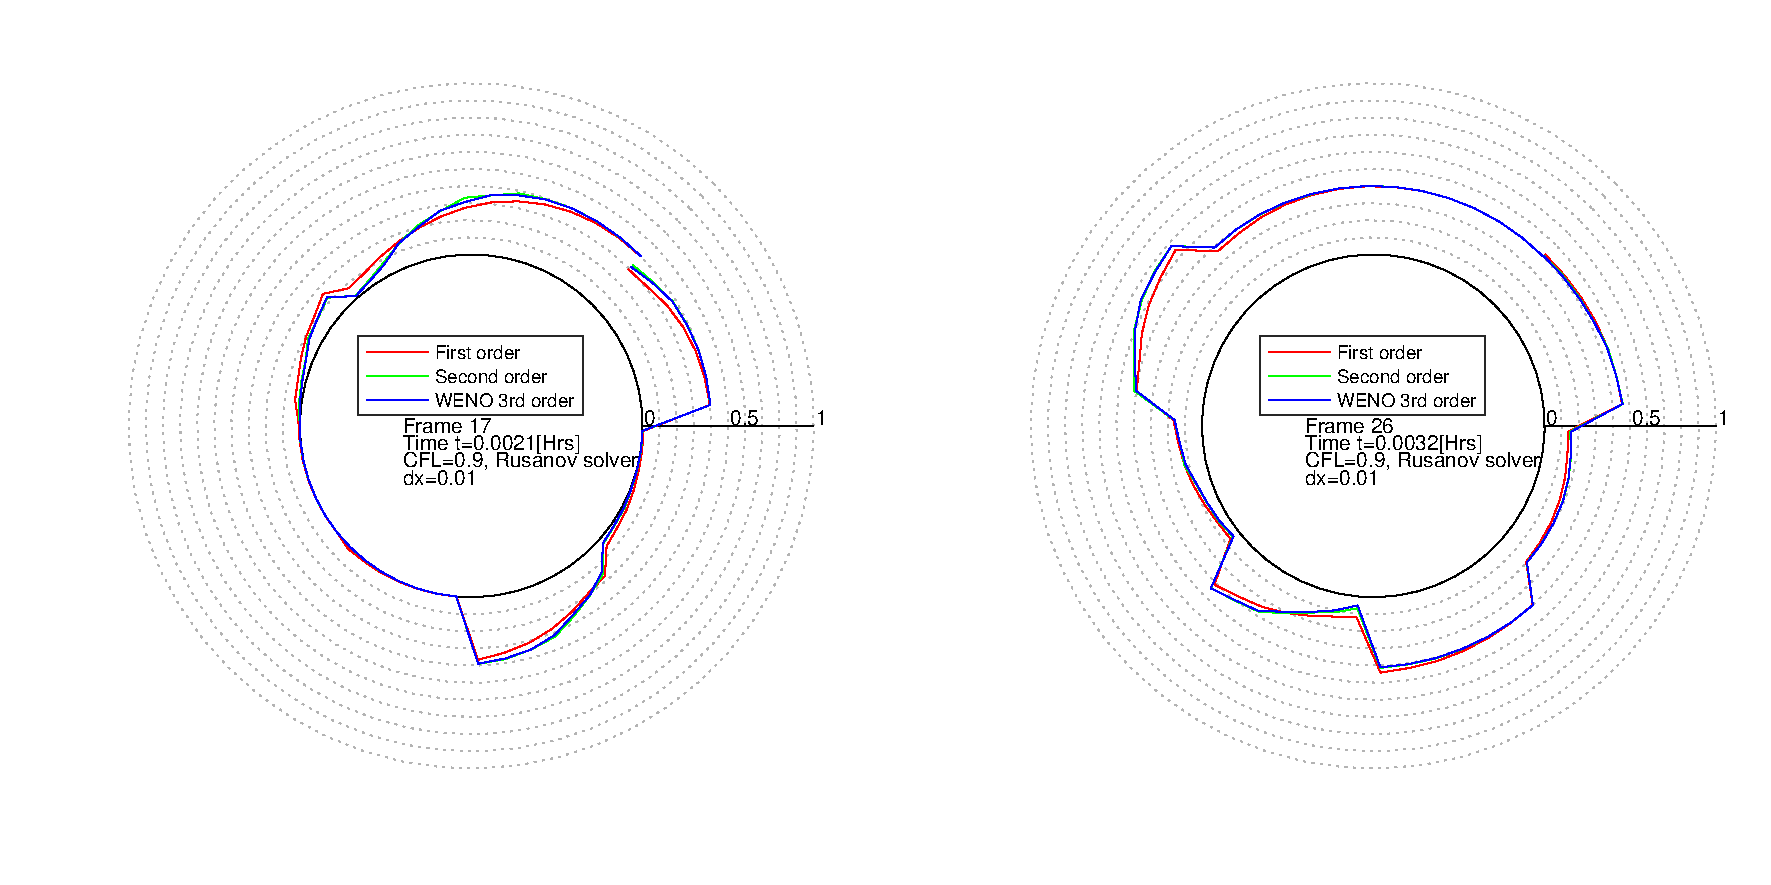
\includegraphics[trim=60 55 20 40,clip,width=\textwidth]{ReDiRoma_reco.pdf}
		\caption[Re Di Roma : Reconstruction]{Two time steps at frame 17 (left) and 26 (right) of traffic density feeding through the Re Di Roma central roundabout. Lower order reconstruction methods smooth out discontinuities at junctions whereas the higher order methods resolve jumps more accurately.}
		\label{fig:randd:rediroma:reco}
	\end{figure}
	
	\begin{figure}
    		\centering
        		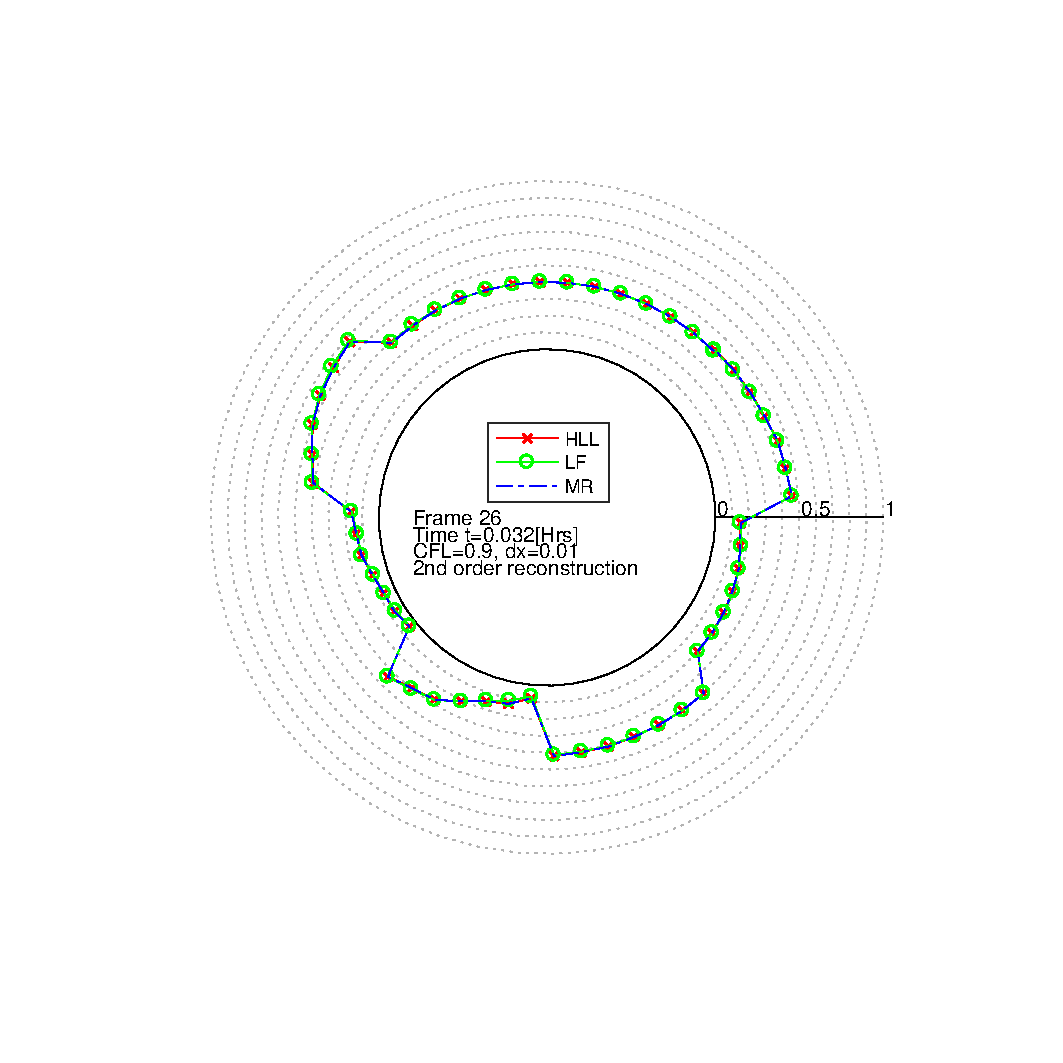
\includegraphics[trim=100 100 80 80,clip,width=0.8\textwidth]{ReDiRoma_riem.pdf}
		\caption[Re Di Roma : Riemann solvers]{The choice of Riemann solver results in a negligible difference in solution. The HLL and Murman-Roe (MR) solver solutions are identical and Lax-Friedrichs (LF) differs only very slightly.}
		\label{fig:randd:rediroma:riem}
	\end{figure}
	
\subsection{Wakefield M1 Junction 40}
\label{sec:randd:M1J40}

	The common simple UK motorway junction meets a crossing A-road at right angles and the model junction can be described by junction 40 of the M1 in Wakefield. Figure \ref{fig:randd:M1J40:map} shows the small interchange network surrounding the meeting of a fast high-density motorway taking traffic to and from London, the Midlands and Leeds. This network is a good example of when a time-dependent TDM may be useful to model over a long time period such as 24 hours. During the morning hours lots of traffic may be coming from all directions towards Leeds, and the opposite in the evening rush hour at high densities. This map has been traced in MATLAB and used for postprocessing (Appendix \ref{code:m1j40})for the initial simulation results, which can be found in Figure \ref{fig:randd:M1J40}. Not only is the line drawing of the motorway junction coloured by high and low local densities, but the higher density regions are matched with a thicker line. This simulation uses first order reconstruction with Lax-Friedrichs numerical flux calculations. Frames from this initial simulation are used to generate the animation \emph{M1J40.mp4}. This figure allows the clear identification of a high local density on the southbound lane of the motorway after traffic rejoins from the A roads and the roundabout slip road. The following results use more classical postprocessing and analyse the influence of the CFL number, and reconstruction around the motorway and slip lanes.
	\\ \\
	The southbound motorway lane and its slip lane off to the junction roundabout are shown in Figure \ref{fig:randd:M1J40:cfl}, with 4 profiles for different values of the CFL constraint which defines the time resolution from the spatial resolution. The main motorway section shows a spike in density just before the slip lane begins, after which the slip lane density begins to increase. This is not as expected and may be due to a fault in the junction solver. In terms of the CFL influence on solution accuracy, lower CFL give rise to a more accurate capturing of the density jump along the motorway section that has not departed off the slip lane. 
	\\ \\
	The spike observed in Figure \ref{fig:randd:M1J40:cfl} cannot be due to the reconstruction interference at junctions as Figure \ref{fig:randd:M1J40:reco} shows the same spike for many reconstruction methods. This figure shows the whole southbound M1 lane with off and on slip roads. The two drops in density at 100 and 170 are due to the inlet flow of the southbound motorway not leaving the off-slip road, and flow from the A road joining the motorway from the on-slip road respectively. The 5$^{th}$ order WENO scheme gives a small increase before the main drop in density, this is not seen in the 3$^{rd}$ or bounded 7$^{th}$ schemes. The 3$^{rd}$ order MUSCL scheme appears to be less accurate than the 2$^{nd}$ order, which from Figure \ref{fig:randd:traffic_circles:limiters} we can conclude that with a more sensible choice of slope limiter, the 3$^{rd}$ order MUSCL scheme will behave better. A different slope limiter may also reduce some of the oscillations in the density drop with this MUSCL reconstruction. We can also see that the smaller drop in density from 0.3 to 0 gives rise to a less smooth 7$^{th}$ order WENO reconstruction, when compared to the larger earlier jump. 
	
	\begin{figure}
    		\centering
        		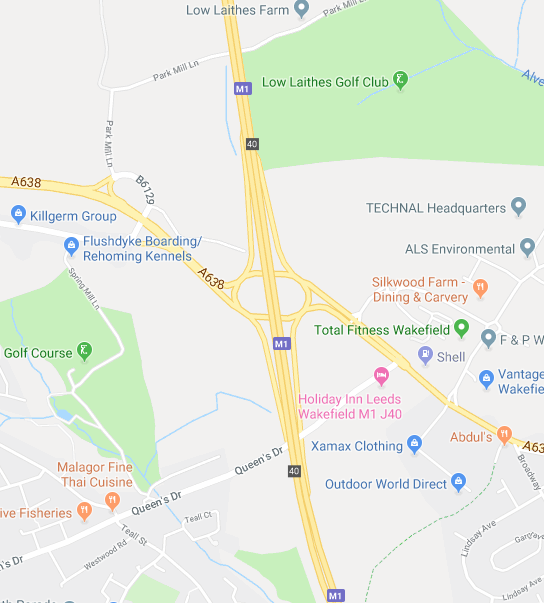
\includegraphics[trim=0 0 0 0,clip,width=0.58\textwidth]{M1J40.png}
		\caption[Wakefield M1J40 : Junction area map]{Simple and common UK motorway and A-road junction. \emph{Google Maps, 2019.}}
		\label{fig:randd:M1J40:map}
	\end{figure}

	\begin{figure}
    		\centering
        		\subfloat[Developing]{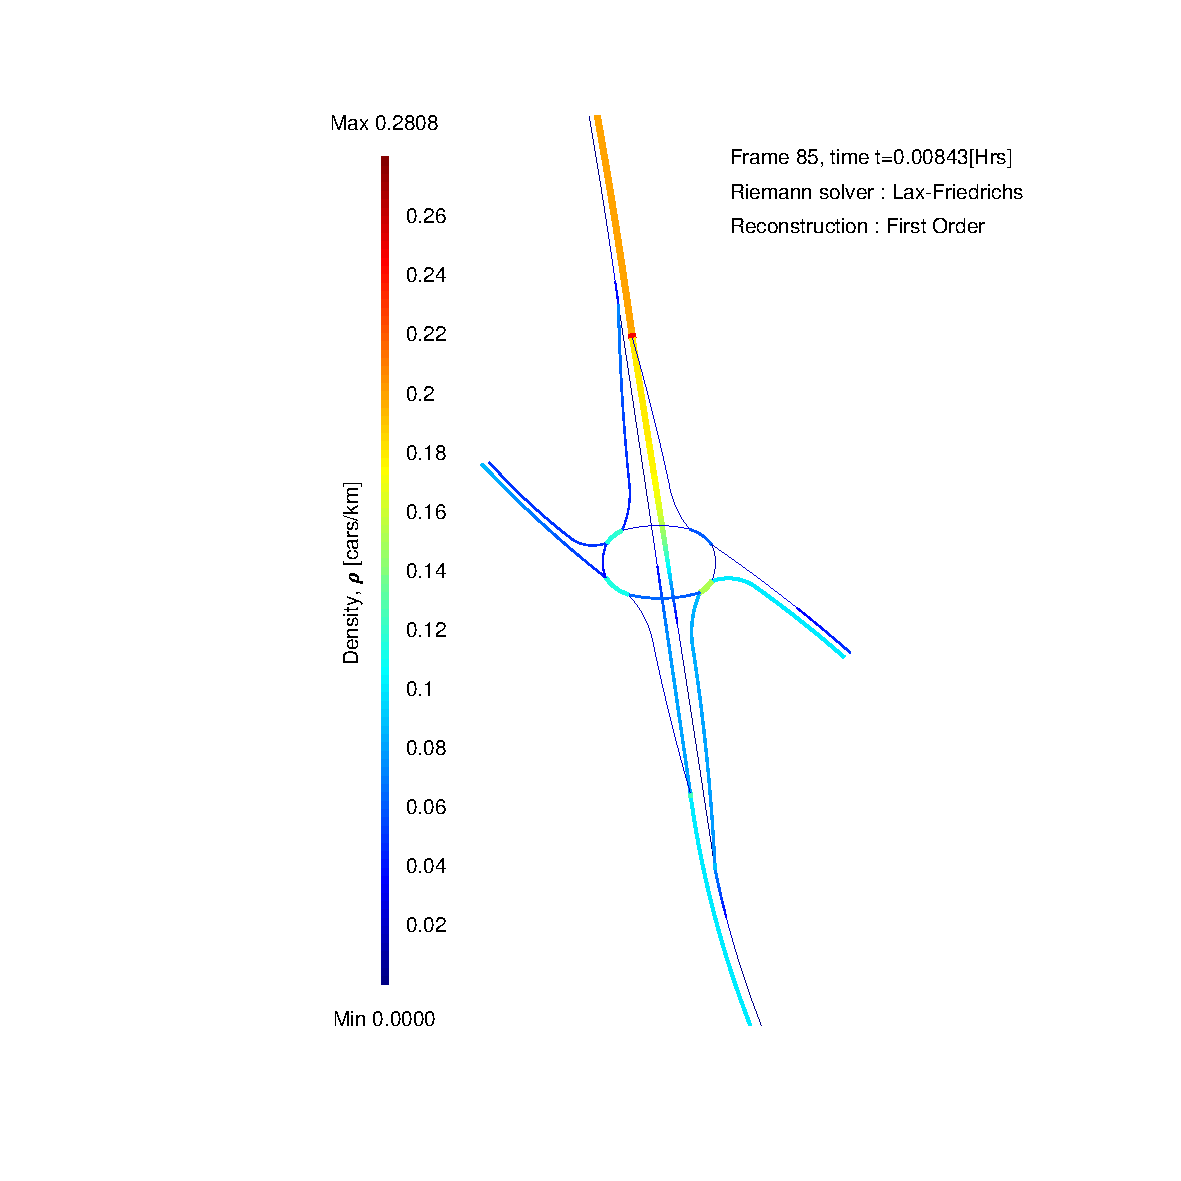
\includegraphics[trim=230 70 70 50,clip,width=0.426\textwidth]{M1J40_1.pdf}\label{fig:randd:M1J40:dev}}
        		\hfill
        		\subfloat[Steady]{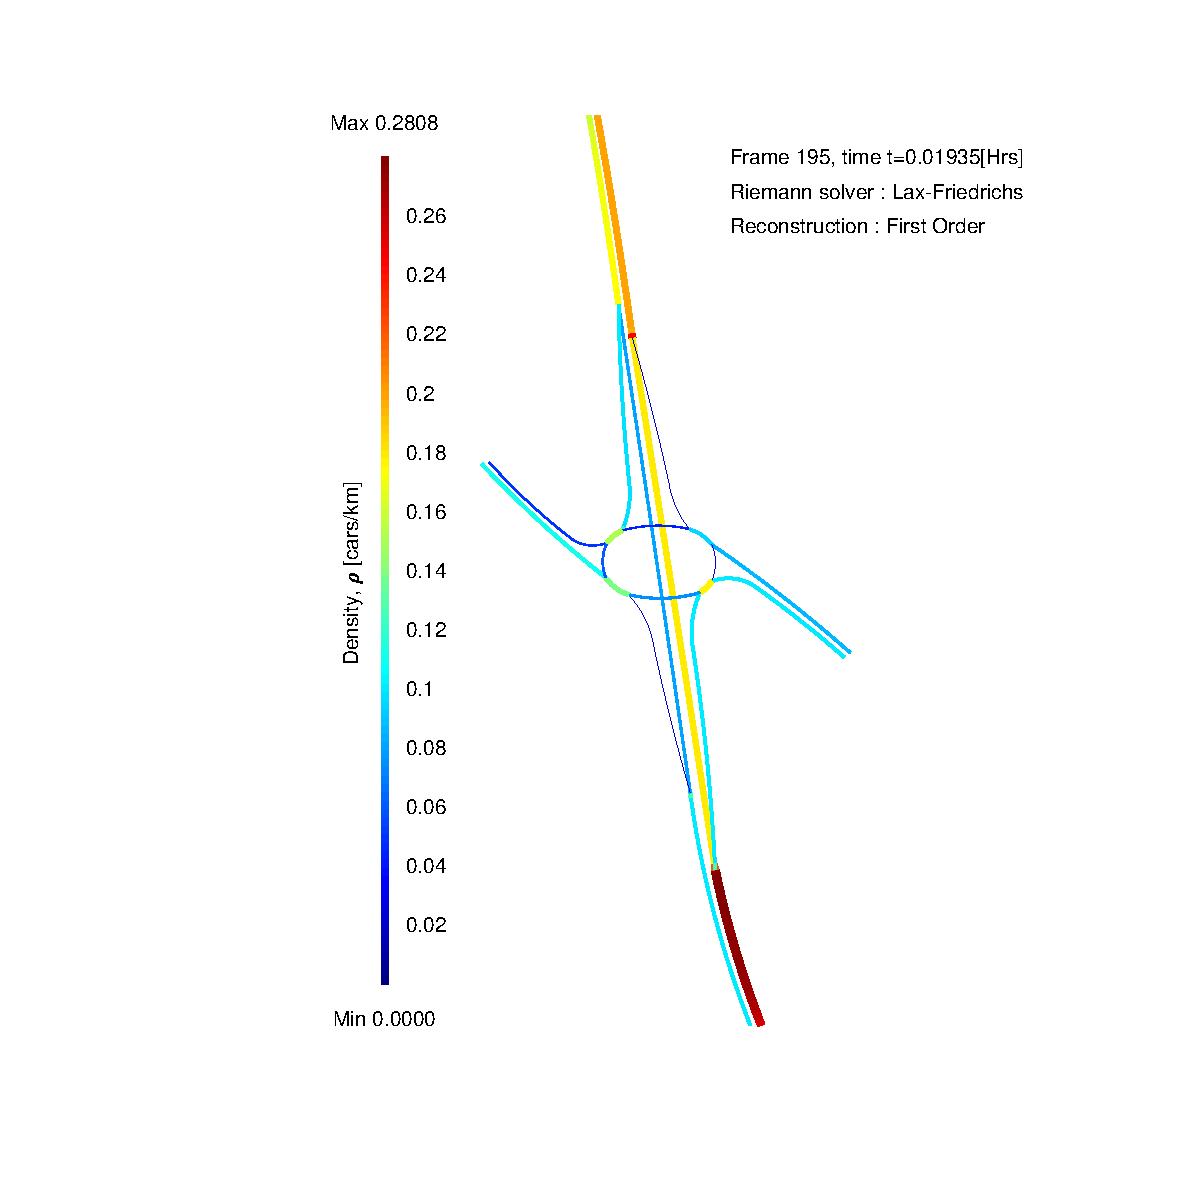
\includegraphics[trim=150 70 70 50,clip,width=0.553\textwidth]{M1J40_2.pdf}\label{fig:randd:M1J40:steady}}
		\caption[Wakefield M1J40 : Density line contour]{Heavy flow southbound from Leeds towards Wakefield and further south. Highlighting the higher density areas of the motorway junction roundabout.\label{fig:randd:M1J40}}
	\end{figure}
	
	\begin{figure}
    		\centering
        		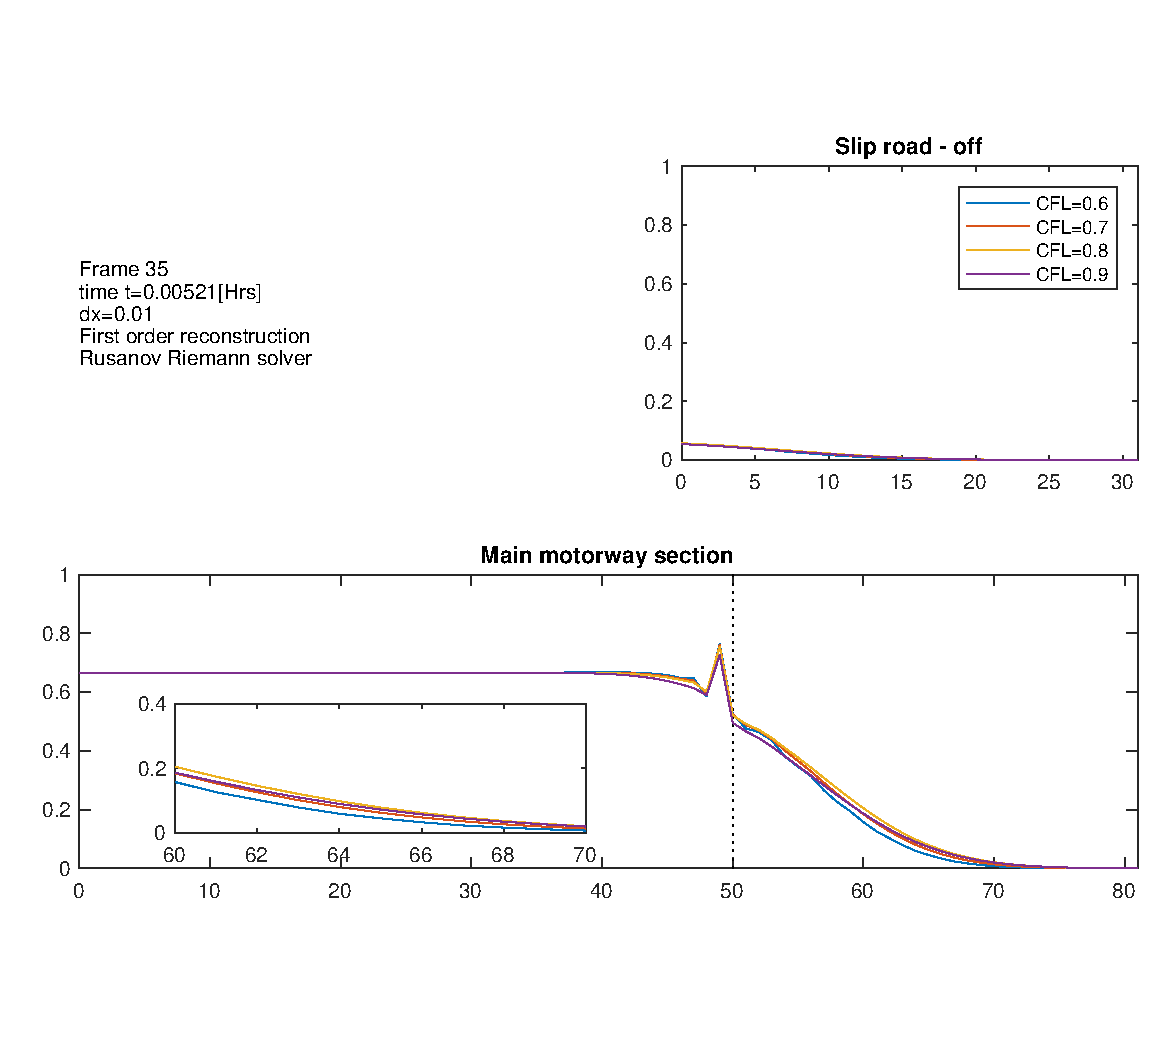
\includegraphics[trim=20 75 10 55,clip,width=0.93\textwidth]{M1J40_cfl.pdf}
		\caption[Wakefield M1J40 : Density profile for varying $CFL$]{The influence of $CFL$ number is little, there are oscillations present at the slip road entrance for all $CFL$. The value $CFL=0.6$ appears to capture the traffic density jump with highest gradient. These simulations are analysed by simulation time in Figure \ref{fig:randd:Time:M1J40_CFL}}
		\label{fig:randd:M1J40:cfl}
	\end{figure}
	
	\begin{figure}
    		\centering
        		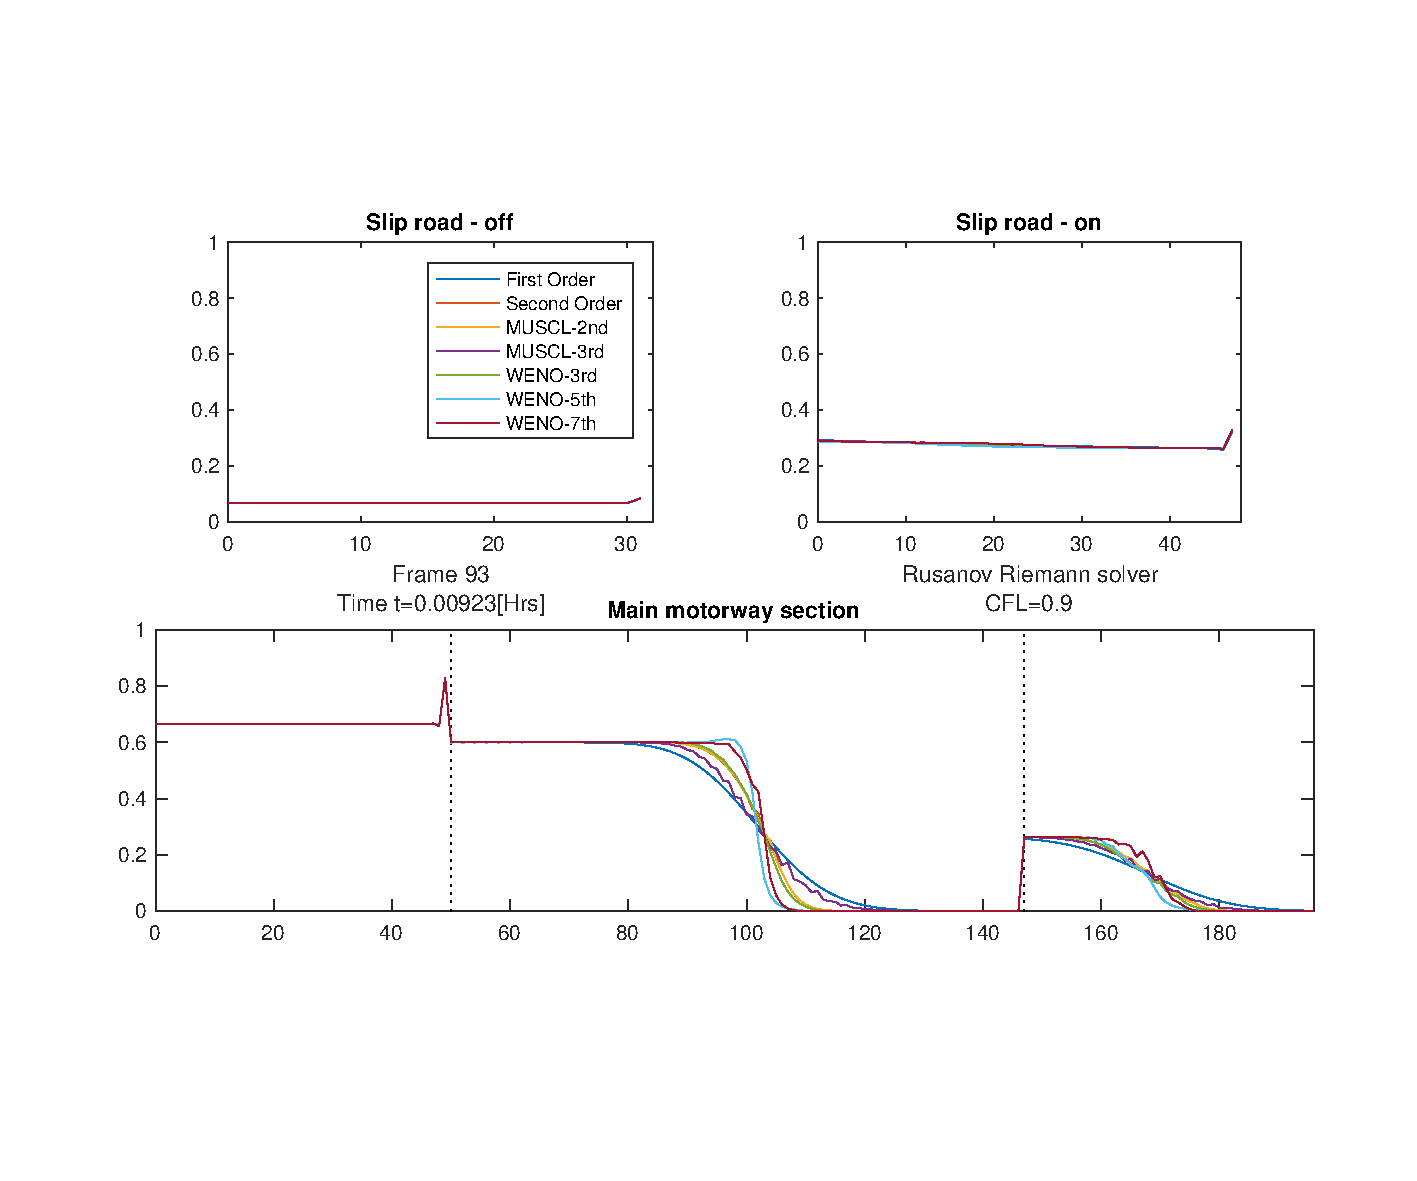
\includegraphics[trim=57 110 40 100,clip,width=\textwidth]{M1J40_reco.pdf}
		\caption[Wakefield M1J40 : Density profile for varying reconstruction]{$dx=0.01$. This figure shows the southbound motorway lane with two slip roads towards and away from the roundabout. Reconstruction appears to have a significant influence on the accurate capturing of a jump in traffic density. The general pattern is a more accurate shock resolution for higher order schemes, however this comes at the cost of computational time and oscillations.}
		\label{fig:randd:M1J40:reco}
	\end{figure}

\section{Time Analysis}
\label{sec:randd:timeanalysis}

	A high resolution numerical scheme can be highly time-costly,  and when such a numerical scheme is coupled with a large road network as the domain this cost is multiplied. It is therefore important to analyse which aspects or parameters of a simulation cause changes in the computational time. The following results are taken from the simulation information output, see Appendix \ref{txt:info:output} , with a total time and a breakdown of the time spent on reconstruction and solving local Riemann problems for example. 
	\\ \\
	The analysis of the 7$^{th}$ order WENO scheme in Section \ref{randd:singleroad} and Figure \ref{fig:randd:single:7thOrder} is followed by Figure \ref{fig:randd:Time:SingleRoadW7}. This shows how the higher order WENO schemes vary in terms of total simulation time (orange) and the time-breakdown on simulations of the single road segment. With high resolution reconstruction methods, the reconstruction time will dominate the simulation and the total time is reflected by this. The unbounded 7$^{th}$ order scheme saves time over the bounded solution by not computing the bounds themselves, but as seen in Figure \ref{fig:randd:single:7thOrder} this saving is not worth the cost of a meaningless solution. The monotonic bounding from Balsara and Shu \cite{BalsaraShu00} is essential for the 7$^{th}$ order WENO reconstruction.
	\\ \\
	The alternate MUSCL reconstruction method also has an important parameter which contributes to both computational speed and solution accuracy. The MUSCL slope limiter as in Section \ref{sec:HRS} and Appendix \ref{ap:MUSCLslopelim} is a simple tool such that can easily be written into any program to be varied and tested for solution (Figure \ref{fig:randd:traffic_circles:limiters}) and in Figure \ref{fig:randd:Time:traffic_circles:limiters}, for computational time. We identified the Monotonised Central \cite{VanLeer77} and UMIST \cite{Lien94} limiters as the most admissible in terms of density jump capturing accuracy on the traffic circles network, and in this figure it is clear that these two schemes increase the computational cost. The VanLeer \cite{VanLeer74} limiter can be seen here to be one of the quickest, and in Figure \ref{fig:randd:traffic_circles:limiters} is identified as a high accuracy limiter with a smooth and high gradient density drop. This figure also shows the difference in cost when limiters are applied to the 2$^{nd}$ or 3$^{rd}$ order MUSCL schemes, of which all limiters show a similar small increase in time and all 3$^{rd}$ order total times are greater than 3$^{rd}$ order totals as expected. The VanLeer \cite{VanLeer74} limiter however has a slightly smaller 3$^{rd}$ order speed-up.  
	\\ \\
	The final time analysis from the traffic circles network is that of spatial resolution, the time taken for solutions shown in Figure \ref{fig:randd:traffic_circles_dx} and more values of $dx$ are simulated and the time breakdown is shown here in Figure \ref{fig:randd:Time:traffic_circles:grid}. It is expected that with a finer spatial resolution, the road network is described by a greater number of computational cells which will result in more calculations and a greater simulation time. With a second order reconstruction it is interesting to see that it is the local Riemann solutions that begin to dominate the total simulation time for the smallest $dx$ simulated here. At the largest $dx=0.175,0.2$ the reconstruction and flux times appear very similar. As with most numerical simulations there is a compromise between solution accuracy and computational time, here a value of $dx=0.05$ gives a valuable solution and saves 75\% of the $dx=0.025$ simulation time. 
	
	\newpage
	
	\begin{figure}[H]
    		\centering
        		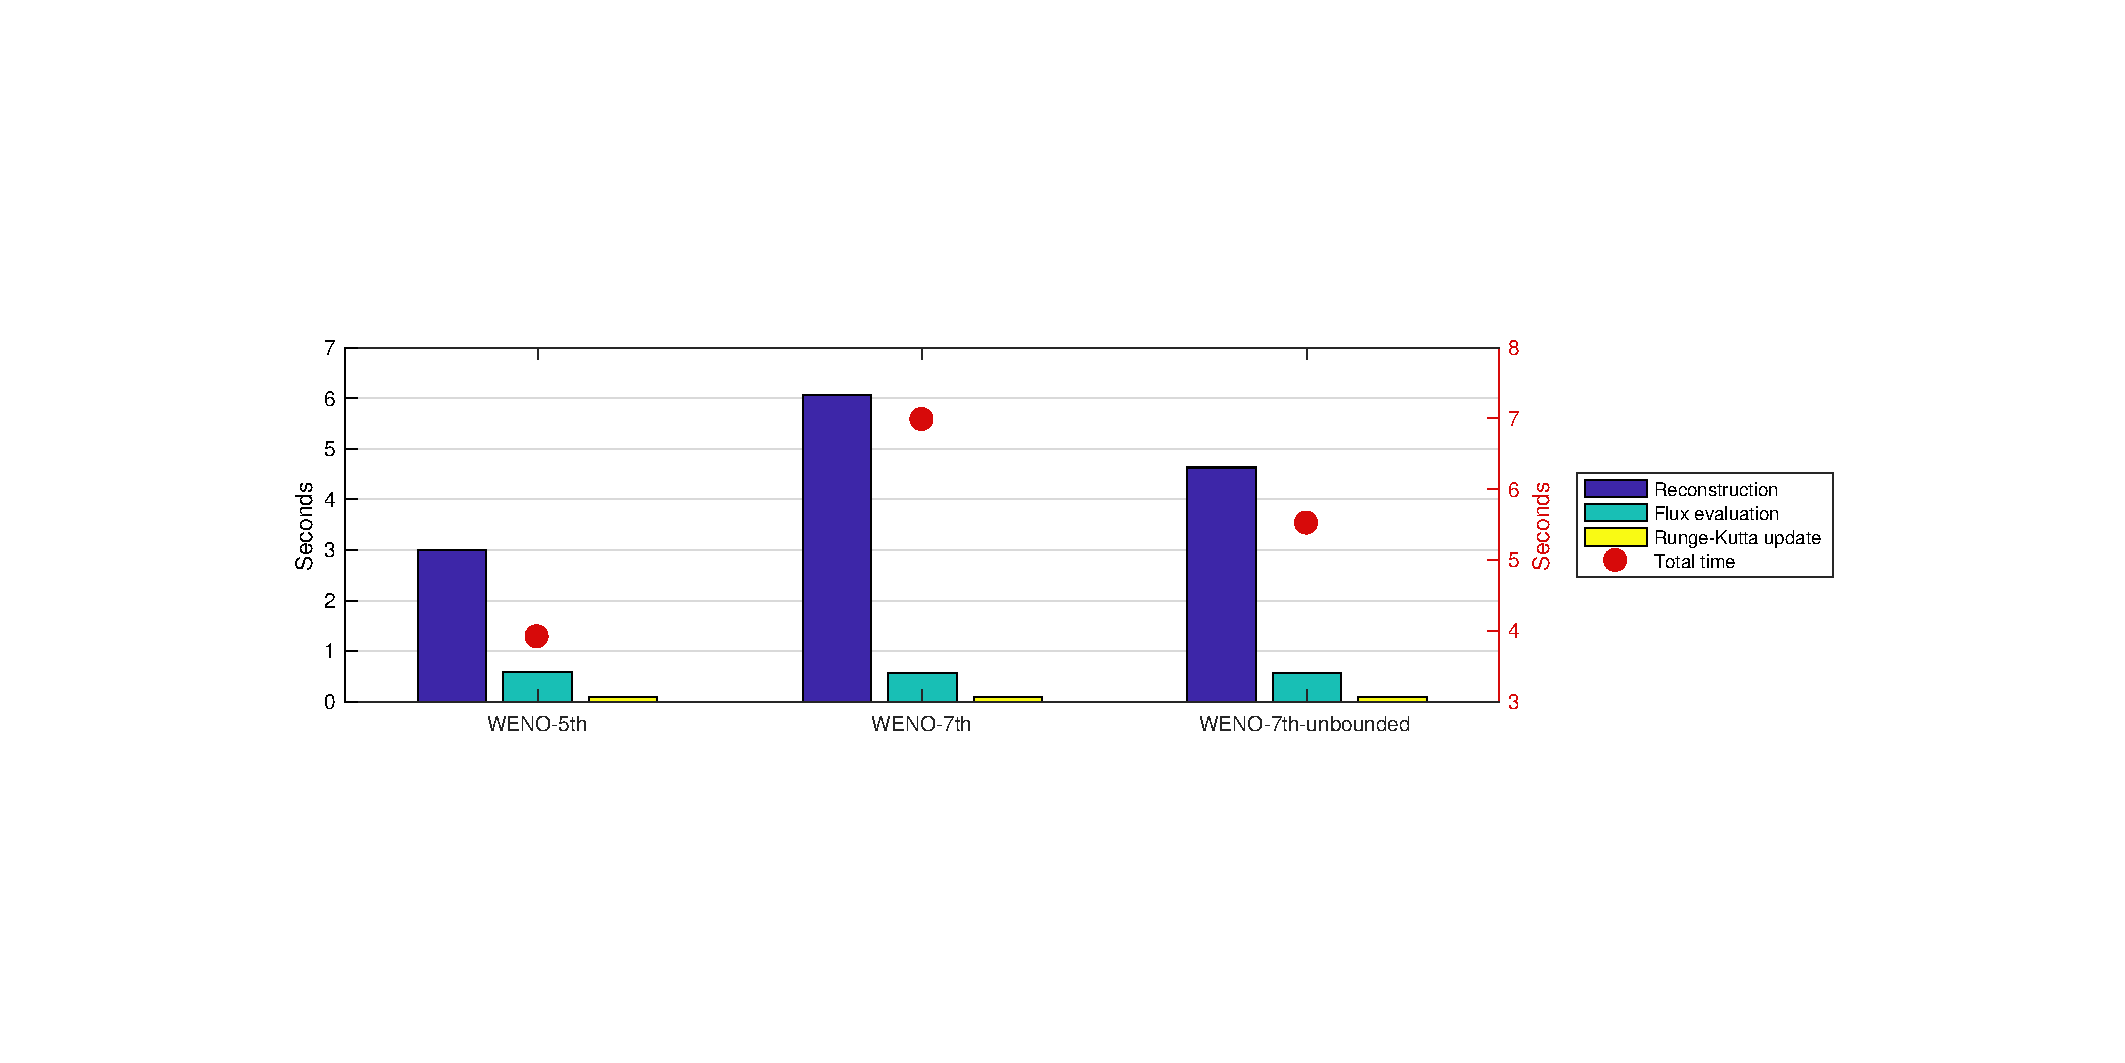
\includegraphics[trim=140 160 138 160,clip,width=\textwidth]{Time_SingleRoad_W7.pdf}
		\caption[Time Analysis : ]{As expected the $7^{th}$ order scheme has an increased computational cost over the $5^{th}$ order due to calculations over an extra stencil. The unbounded scheme is quicker as no monotonic bounds are calculated but at the cost of an inadmissible solution this cost saving is not valuable.}
		\label{fig:randd:Time:SingleRoadW7}
	\end{figure}
	
	\begin{figure}[H]
    		\centering
        		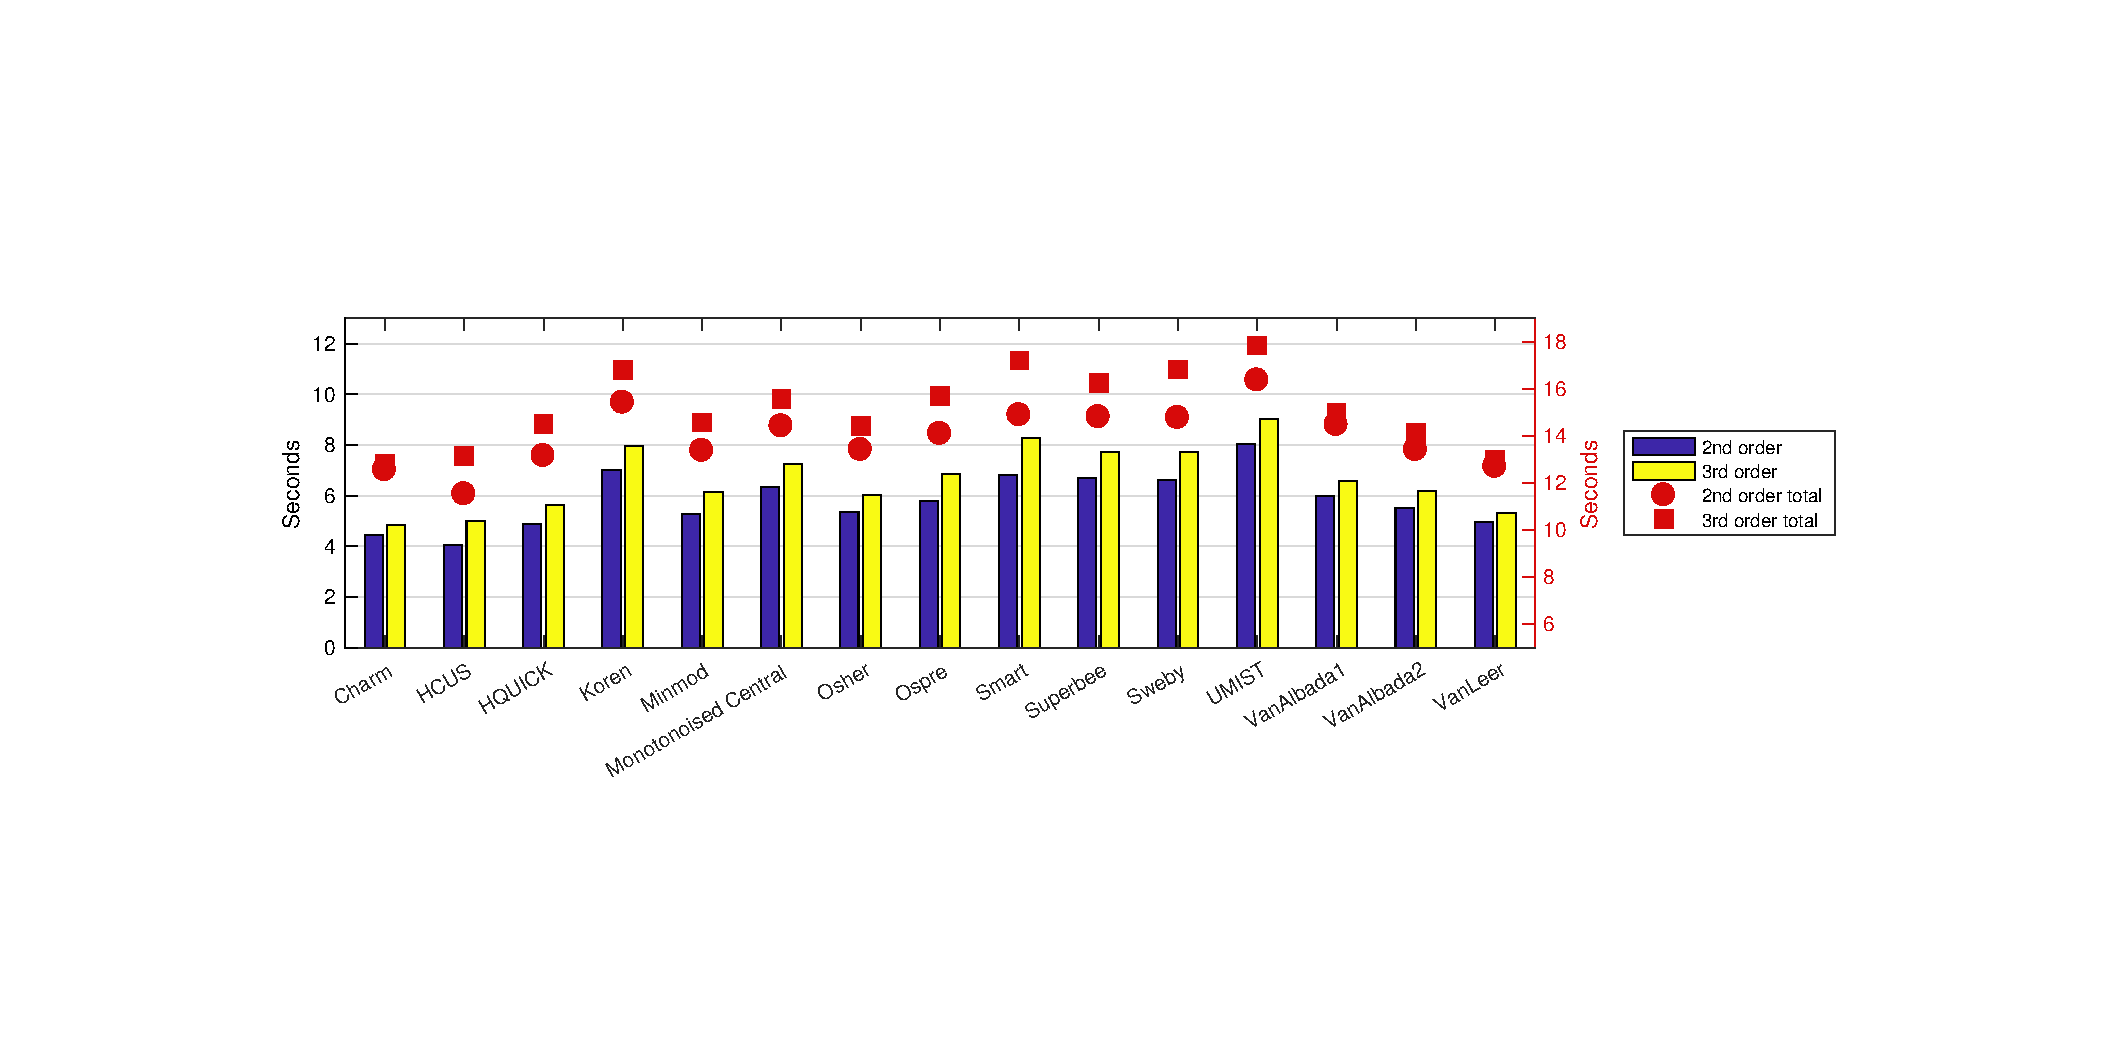
\includegraphics[trim=135 135 135 150,clip,width=\textwidth]{Time_TC_limiters.pdf}
		\caption[Time Analysis : Traffic circle slope limiters]{For all MUSCL slope limiters, the reconstruction time is shown by the bar chart and total simulation with the orange shaped marker. No limiter has a significantly higher time cost with the 3$^{rd}$ order reconstruction.}
		\label{fig:randd:Time:traffic_circles:limiters}
	\end{figure}
	
	\begin{figure}[H]
    		\centering
        		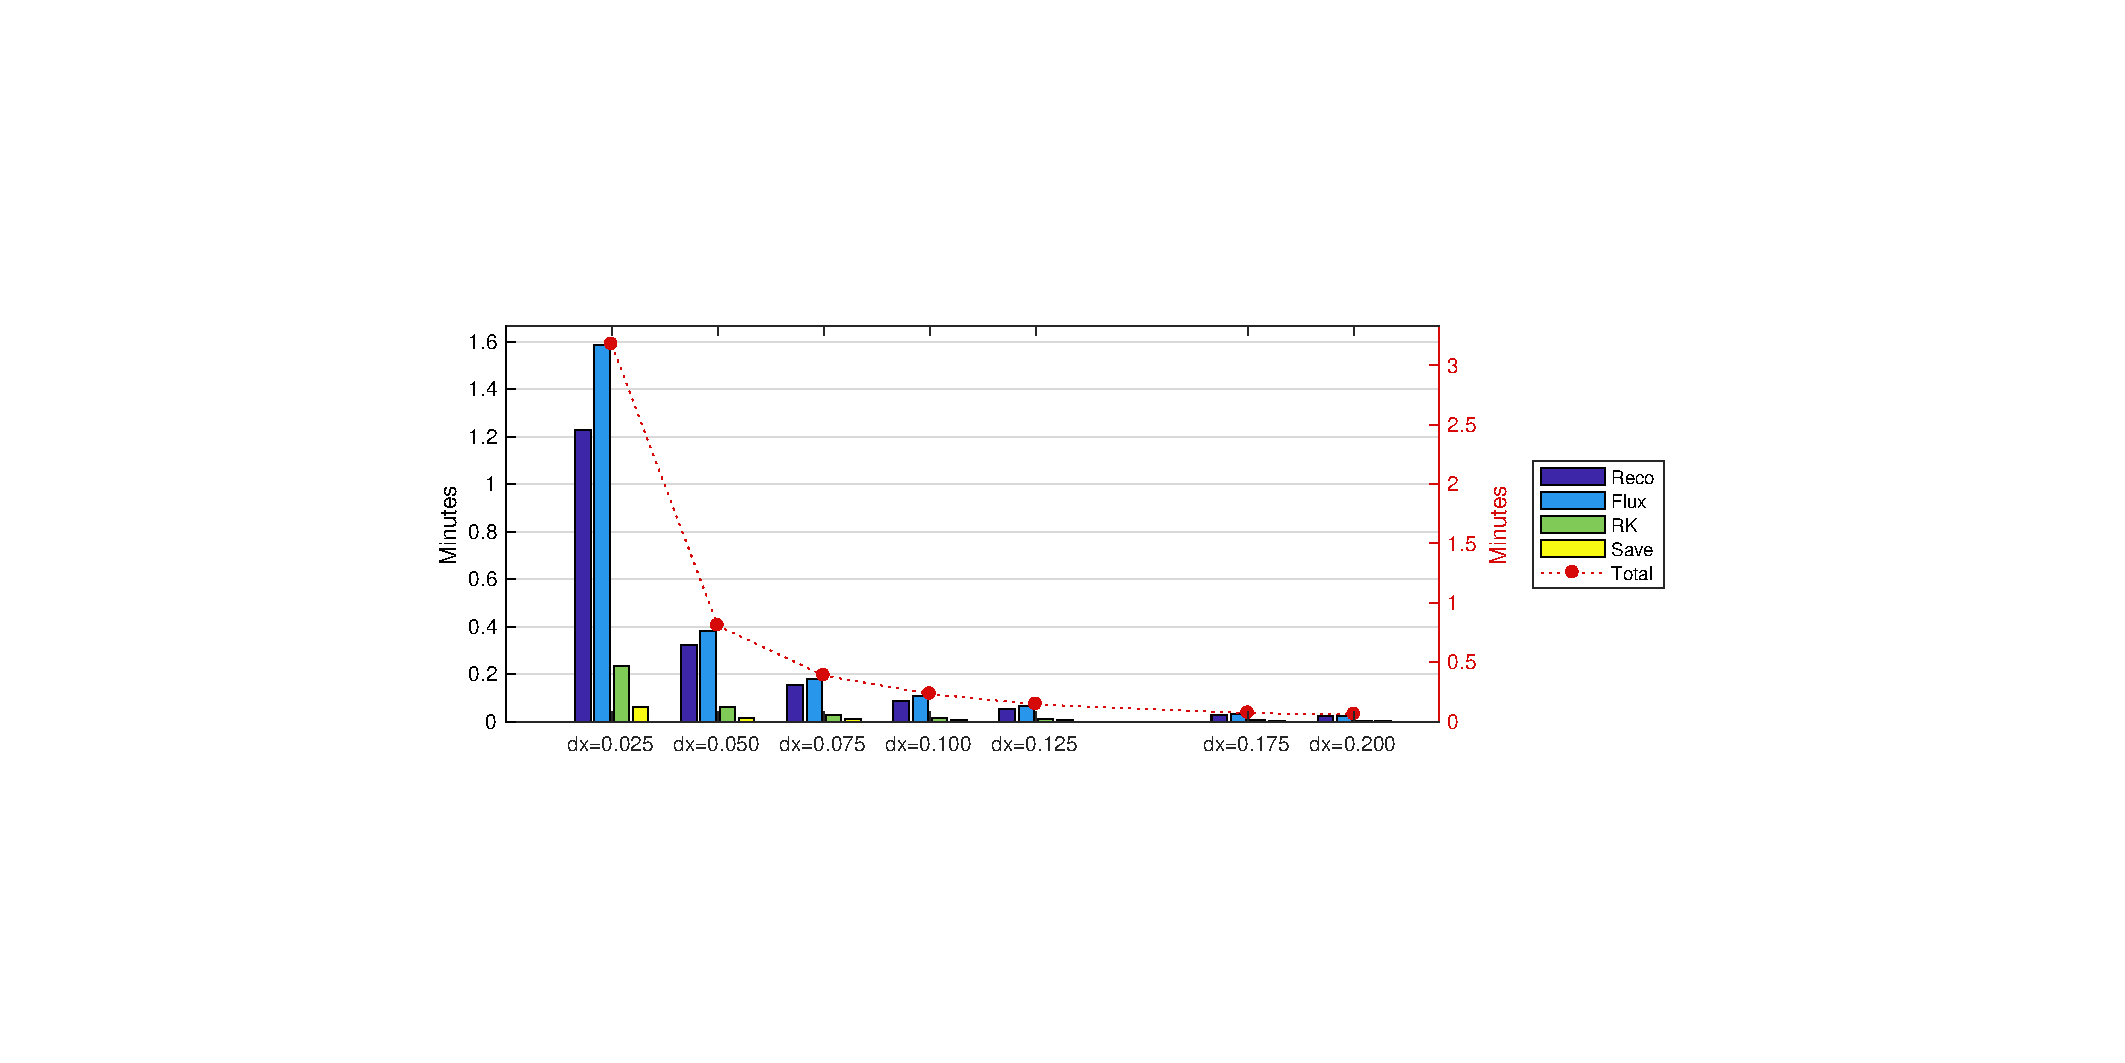
\includegraphics[trim=210 150 220 150,clip,width=\textwidth]{Time_TC_grid.pdf}
		\caption[Time Analysis : Spatial resolution]{A similar time-breakdown shows results including those from Figure \ref{fig:randd:traffic_circles_dx}, and more simulations with varying spatial resolution $dx$.}
		\label{fig:randd:Time:traffic_circles:grid}
	\end{figure}
	
	\pagebreak
	
	\noindent The next figures use time information from solutions of the Wakefield M1 junction simulations. Figure \ref{fig:randd:Time:M1J40_CFL} tests the breakdown of varying the $CFL$ constraint. With a constant $dx$, $CFL\propto dt$, so one would expect lower $CFL$ to give rise to longer computational time. This is the opposite of what is shown in Figure \ref{fig:randd:Time:M1J40_CFL}, computational time increases to a maximum at $CFL=0.8$. At this simulation setup of first order reconstruction with Rusanov flux calculations (see Figure \ref{fig:randd:M1J40:cfl}) the flux evaluations are dominating the total time, but with little difference between density profiles over each $CFL$ it may be wise to use $CFL=0.6$ to save time while also capturing the strongest density gradient along the jump.
	\\ \\
	From the analysis so far, it is not conclusive that the reconstruction influences the simulation time the most. However Figure \ref{fig:randd:Time:M1J40_reco} shows the simulation times for all available reconstruction methods in the solver parameters. With similar times for the 2$^{nd}$ order TVD and MUSCL schemes, generally the higher order reconstruction scheme will take longer to complete the reconstruction process so much that the total simulation time appears similar to the individual reconstruction time bars. After the 1$^{st}$ order scheme, all other methods total times are dominated by their reconstruction. This is as expect as higher order schemes apply extra calculations at each cell, which is multiplied over the total number of cells and time steps. The lower plot shows the relationship of the other simulation processes, these appear independent of the choice of reconstruction.
	\\ \\
	The Re Di Roma roundabout network was simulated for varying Riemann solvers, the solutions shown in Figure \ref{fig:randd:rediroma:riem}, are timed and shown here in Figure \ref{fig:randd:Time:ReDiRoma:riem}. With second order reconstruction, the Riemann solvers crucially can be more or less costly than the reconstruction procedure. In the cases of the Lax-Friedrichs and Murman-Roe solvers the flux evaluation is less costly than reconstruction whereas the HLL solver is slightly more costly than its reconstruction. The total time reflects a combination of these two important simulation procedures. Even though the Murman-Roe solver is quicker than HLL, the total times are similar due to the slower Murman-Roe reconstruction. It is hence clear that at the 2$^{nd}$ order level, the flux evaluations and reconstruction times are not independent and do influence each other. 
	\\ \\
	As with all of the time analysis thus far, it is clear that certain parameters of simulation influence the behaviour and the breakdown of total time into the key simulation sections. Figure \ref{fig:randd:Time:mixed} shows pie charts of the reconstruction, junction solver, flux evaluations, Runge-Kutta update and the saving of simulated data. The only other elements of simulation are road network definition, checking for errors and initialising the density profile, these are omitted from the pie charts as they are of the scale of $10^{-3}$ smaller than the smallest main element, the junction solver. The Wakefield motorway junction network solution with second order reconstruction (top-left) shows how dominating the reconstruction process can be, compared to a first order reconstruction process (top-right). The lower pie shows the increased flux evaluation time with the smallest grid on the traffic circles network tests. 

	\begin{figure}
    		\centering
        		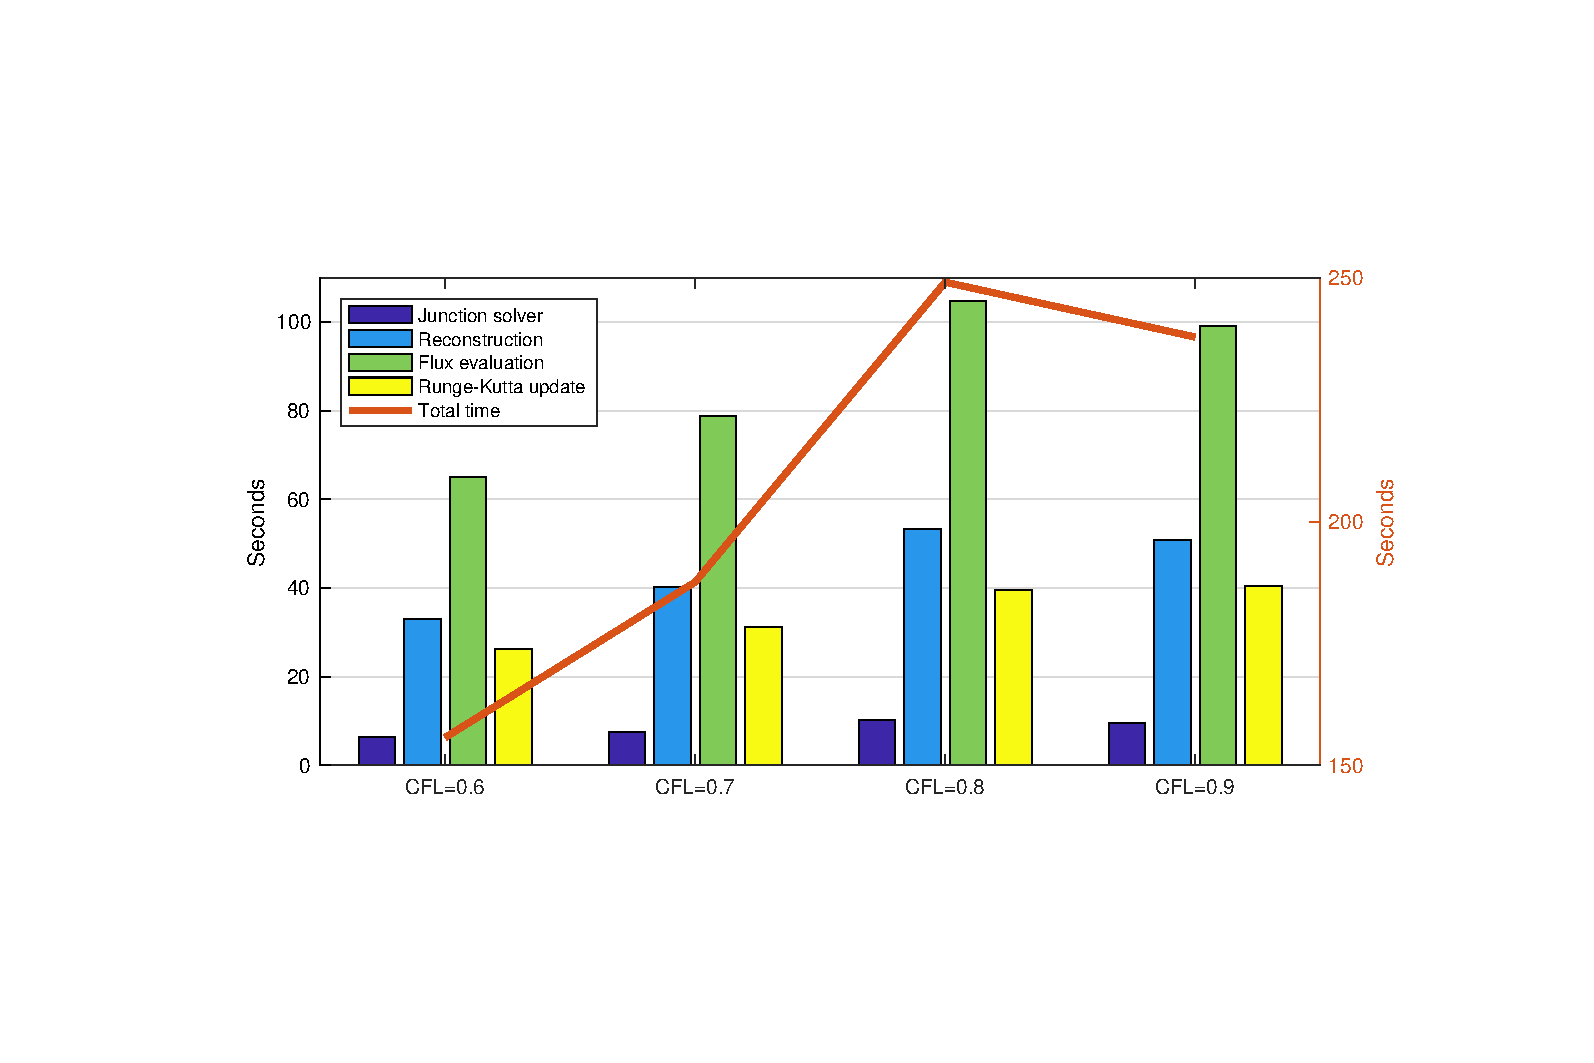
\includegraphics[trim=110 120 90 120,clip,width=\textwidth]{Time_M1J40_CFL.pdf}
		\caption[Time Analysis : M1J40 CFL]{Higher $CFL$ number increases computational time in total and is reflected over all timed segments of the code. The higher $CFL=0.8,0.9$ show a slightly opposite pattern. This information is joint with density profiles in Figure \ref{fig:randd:M1J40:cfl}.}
		\label{fig:randd:Time:M1J40_CFL}
	\end{figure}
	
	\begin{figure}
    		\centering
        		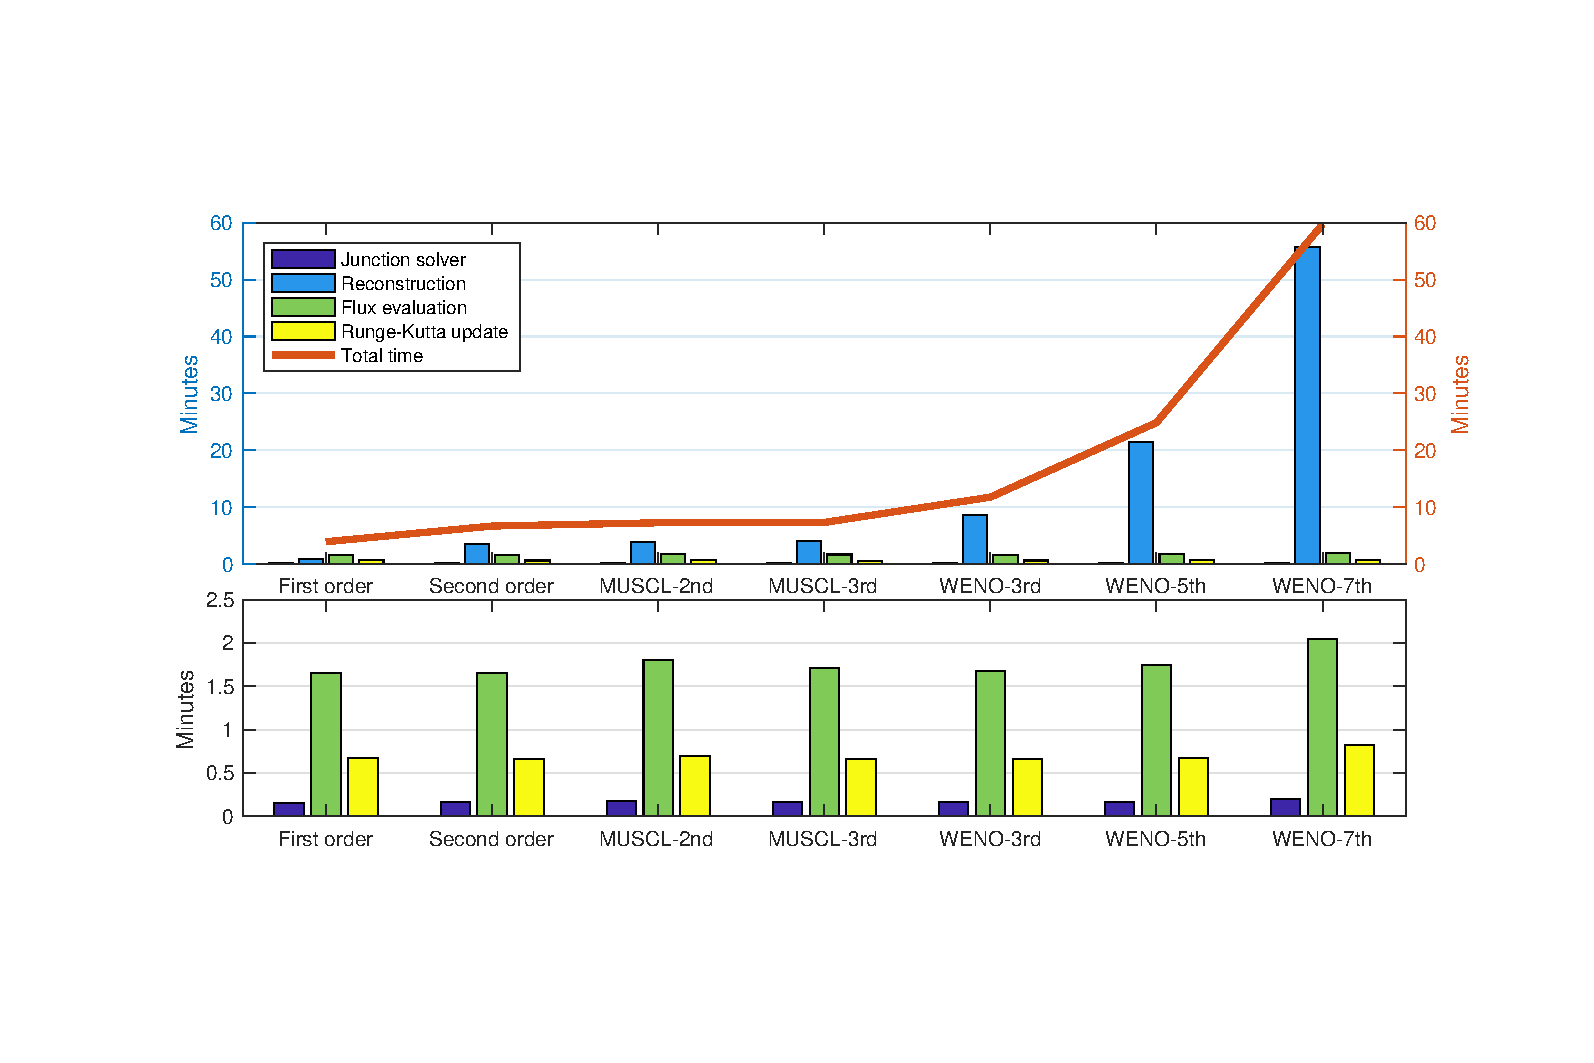
\includegraphics[trim=80 100 60 90,clip,width=\textwidth]{Time_M1J40_reco.pdf}
		\caption[Time Analysis : M1J40 reconstruction]{As reconstruction applies to every cell at every time step, any extra calculations computed as part of the reconstruction process scales with the number of spatial and time steps. Here it is clear that higher order reconstructions increase the reconstruction time (above), and the other simulation processes are unaffected by this (below). }
		\label{fig:randd:Time:M1J40_reco}
	\end{figure}
	
	\begin{figure}
    		\centering
        		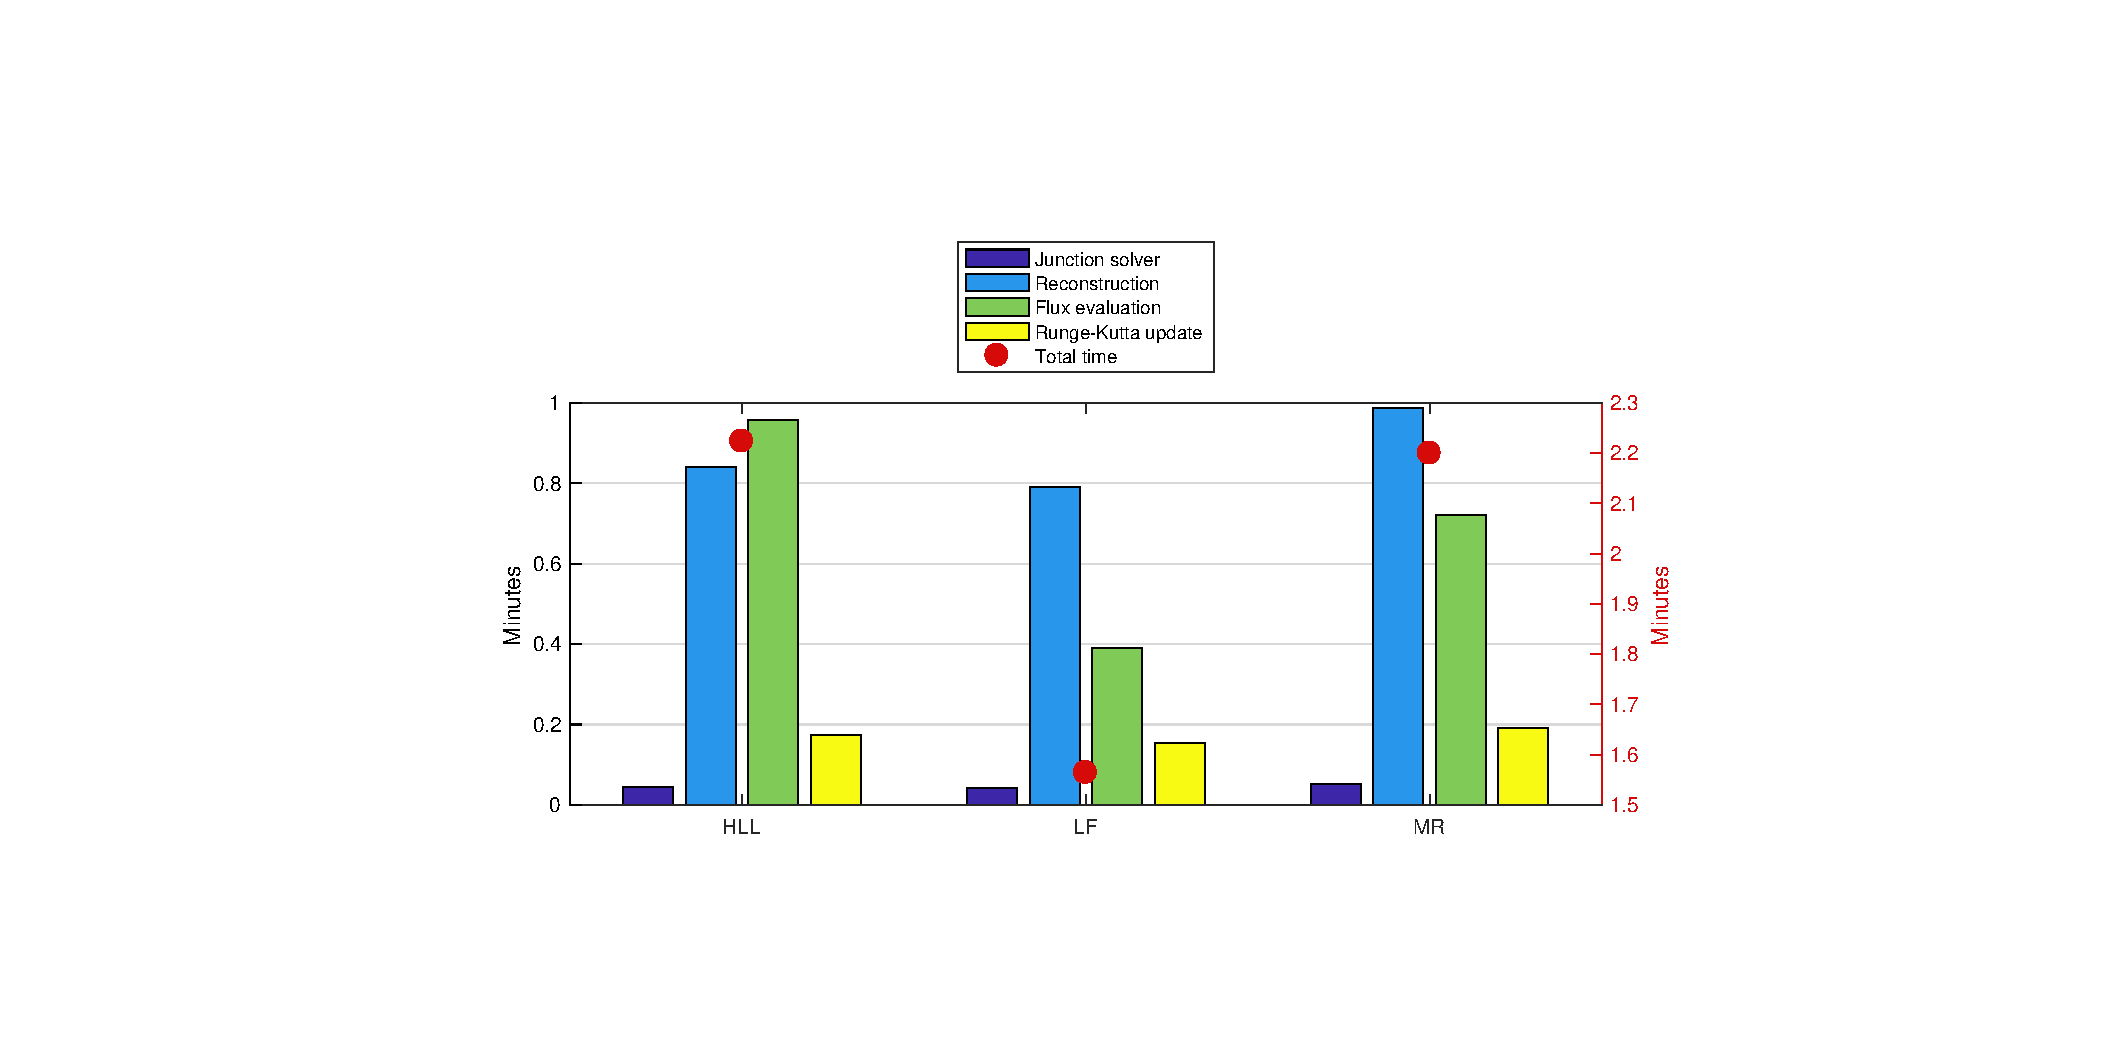
\includegraphics[trim=230 110 210 110,clip,width=0.85\textwidth]{Time_ReDiRoma_riem.pdf}
		\caption[Time Analysis : Re Di Roma Riemann solvers]{The Lax-Friedrichs solver is just over half as quick as the HLL and Murman-Roe solvers. If the choice of Riemann solver has little effect then it may be sensible to minimise computational time with the Lax-Friedrichs solver. }
		\label{fig:randd:Time:ReDiRoma:riem}
	\end{figure}
	
	\begin{figure}
    		\centering
        		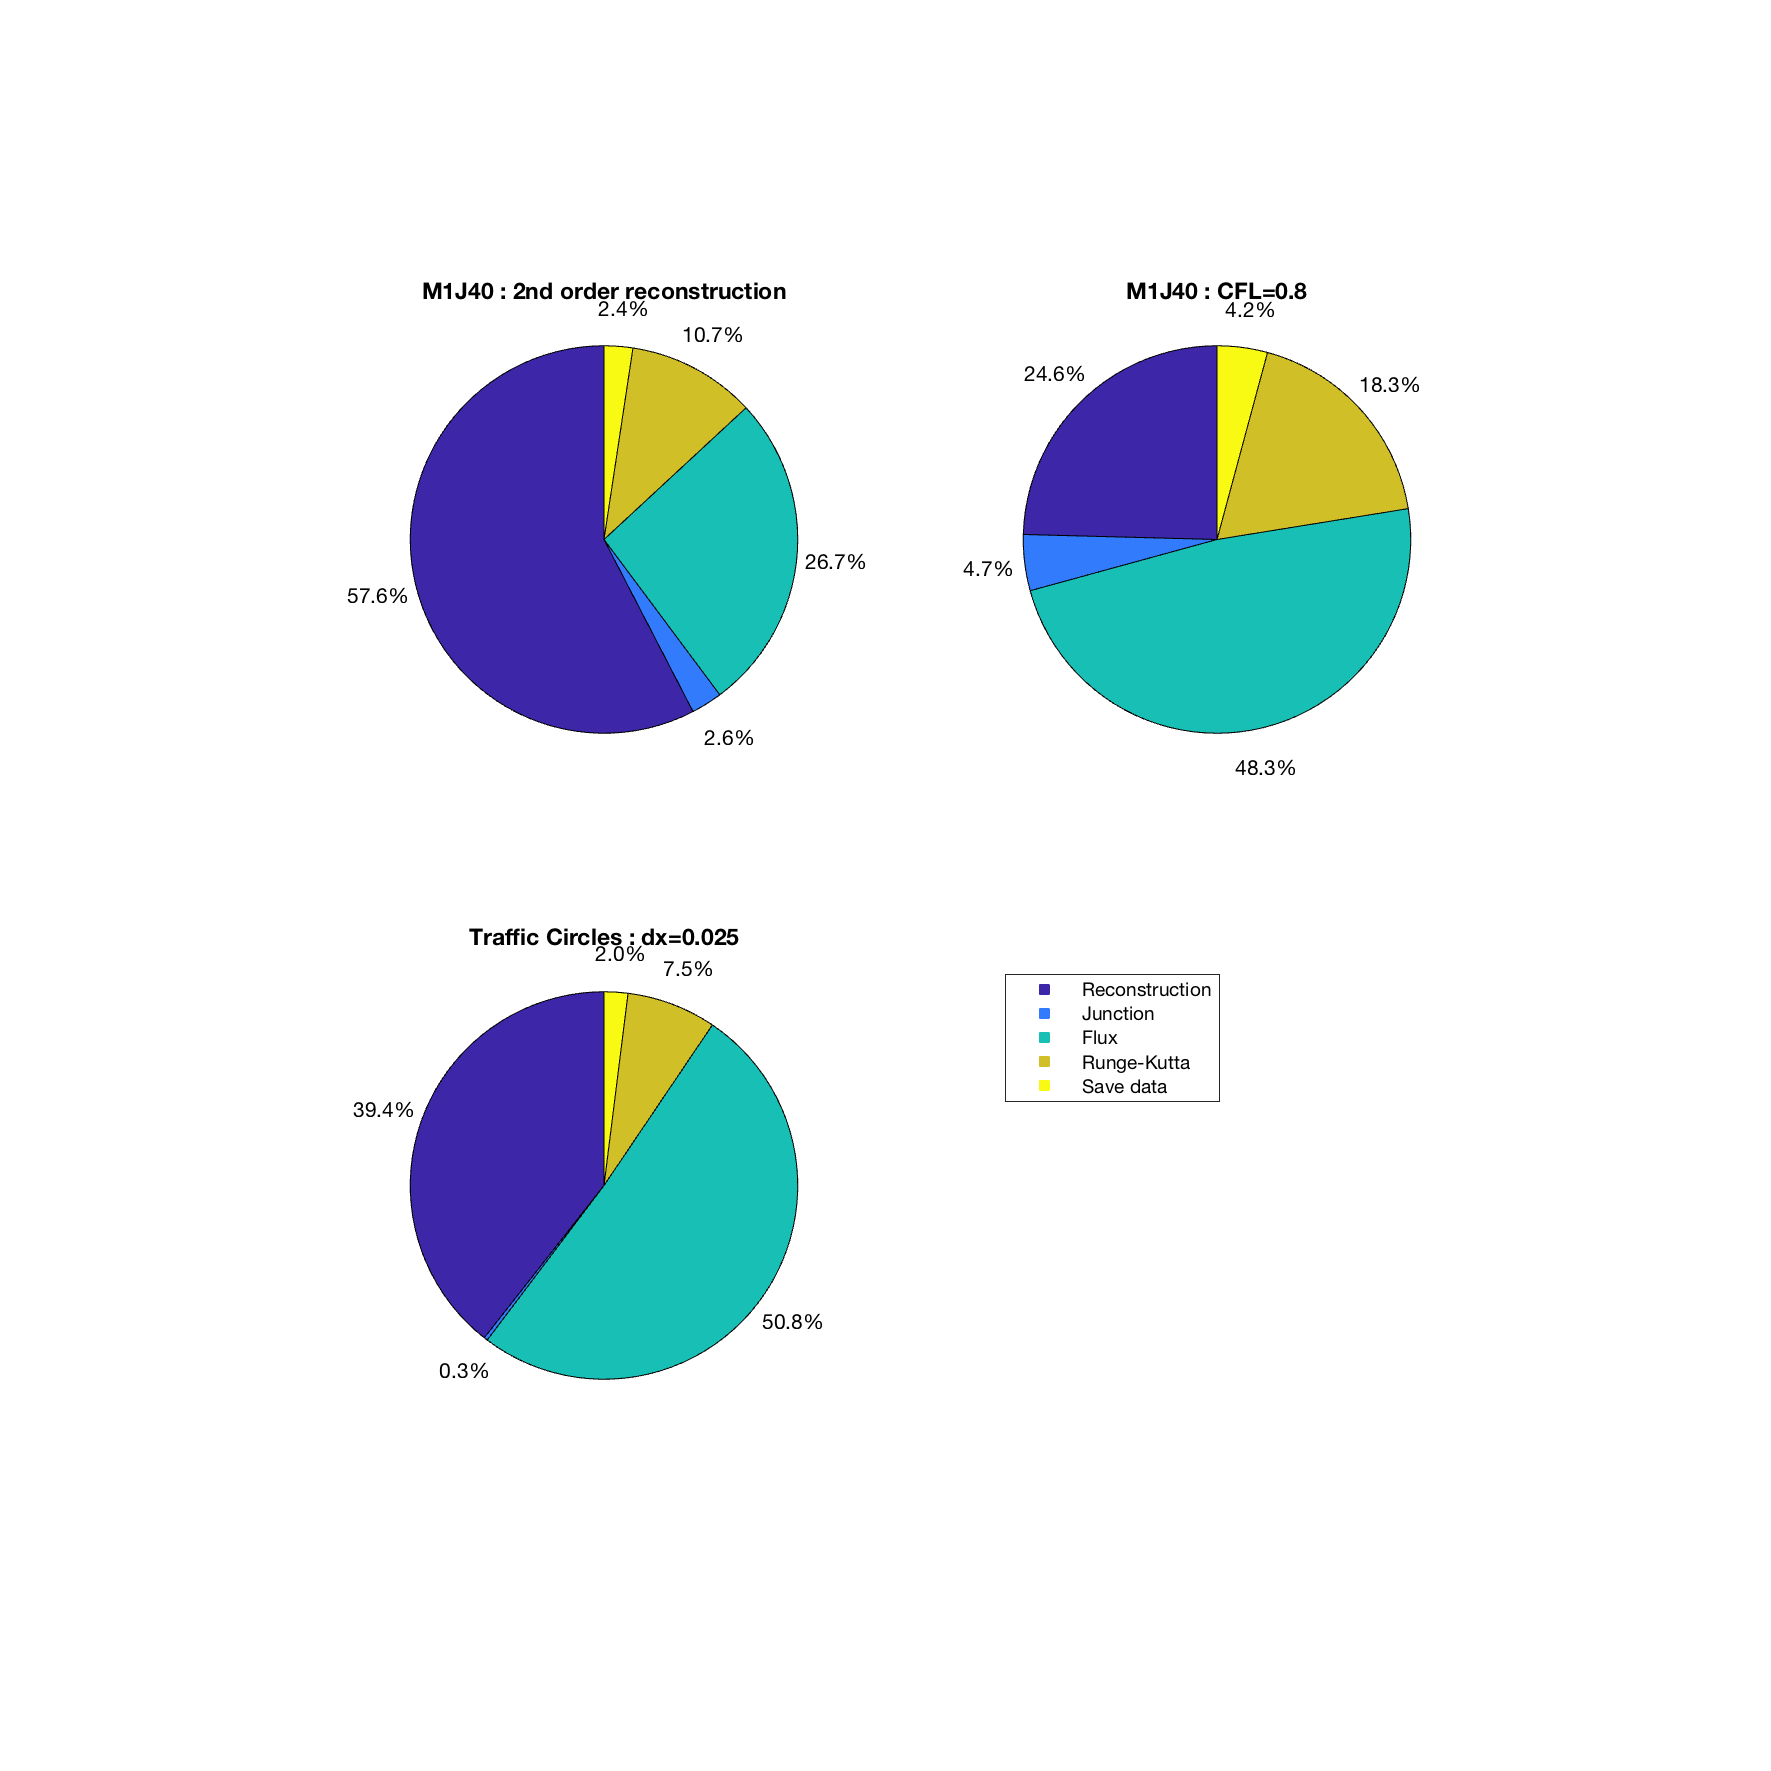
\includegraphics[trim=160 170 160 130,clip,width=0.85\textwidth]{Time_mixed.pdf}
		\caption[Time Analysis : Total time breakdown]{Depending on the choice of simulation parameters, the total simulation time is distributed varyingly over the sections shown in the above legend. For higher order reconstruction, this can dominate almost entirely, but other elements of the simulation are more time-influential with low order reconstructions.}
		\label{fig:randd:Time:mixed}
	\end{figure}
	
	
	
	
	
	
	